\section{Local minimums}
\par Now we want to start studying the unconstrained optimisation problems. The optimisation problems are always conducted over a set of values, and the most simple form of optimisation problems are those whose sets are not constrained at all. Thus the name of \textit{unconstrained} optimisation.
\par The problem that we deal with is typically described by the following syntax:
\begin{equation}
    f_* = \min \{f(x) : x \in \mathbb{R}^n\}
\end{equation}
\par In these kind of problems only the objective function accounts. Since the set is unbounded, the Weierstrass theorem cannot be applied. Many problems in Machine Learning are of this very kind. Thus, these problems are quite important to study. Moreover, the things that we are going to develop will also be very important for the more difficult version of optimisation problems, that is the constrained version. You need to be able to do the unconstrained optimisation in order to do the constrained optimisation.
\par Note that in unconstrained optimisation, the set over which the function is defined is the whole space $\mathbb{R}^n$. This implies that we cannot use Weierstrass theorem.
\par If we aim to find a global minimum of a problem that does not have any special property, is a very hard to solve. Even when we know that a function admits a global minimum, it may be very hard to recognise it. Actually this is usually the major problem. Detecting \textit{a} minimum may be easy, recognising (proving that it is actually a global minimum is what is difficult (see figure \ref{fig:chapter2-many_minimums}). We won't touch this argument in this course, but for not fainted heart look into globalisation techniques.
\begin{figure}
    \centering
    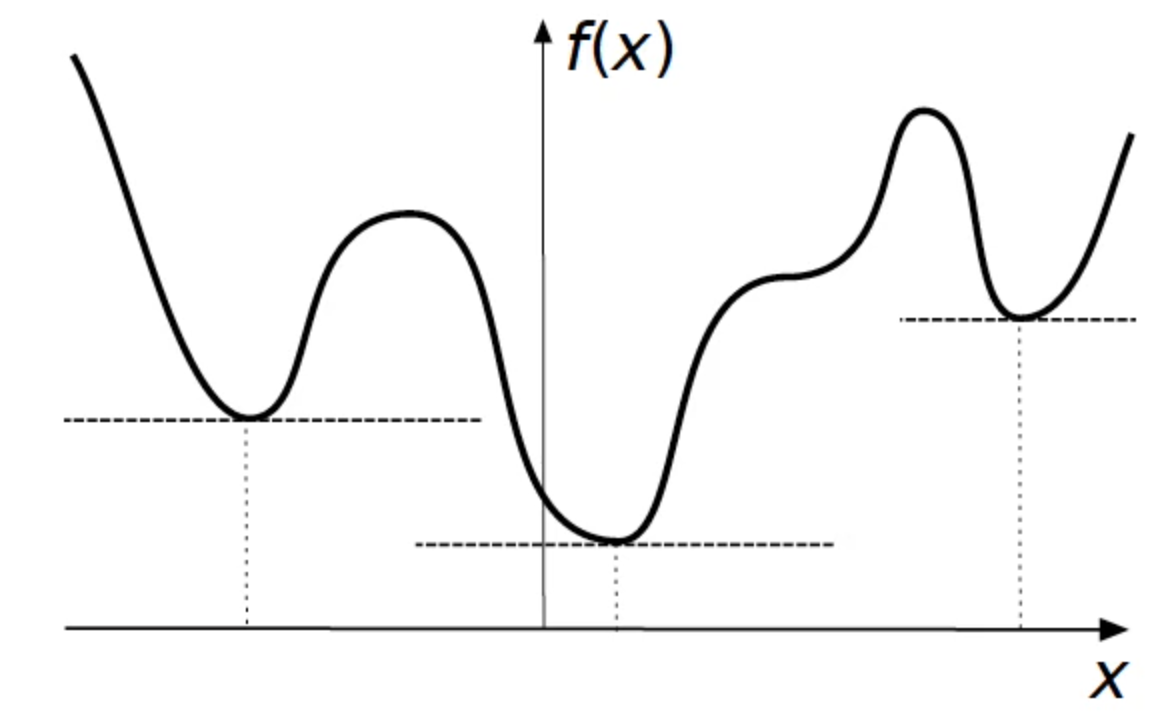
\includegraphics[scale=0.3]{figures/2/chapter2-many_minimums.png}
    \caption{There are different minimums, which one is local and which one is global? It depends where we start looking for it.}
    \label{fig:chapter2-many_minimums}
\end{figure}
\par For this reason, we usually start simple and small: find a local minimum. We say that $x_*$ is a local minimum if it solves the problem:
\begin{equation}
    \min \{f(x) : x \in \mathcal{B}(x_*,\epsilon)\}
\end{equation}
for some $\epsilon > 0$. We say it is a strict local minimum if: $f(x) < f(y)\ \forall y \in \mathcal{B}(x_*,\epsilon)$.
\par If the objective function $f$ is differentiable, then we already know how to compute it. If $x_*$ is a local minimum then its first order derivative (the gradient $\nabla$) is zero:
\begin{equation}
    x^* \textit{ is local minimum} \Rightarrow \nabla f(x^*) = 0
\end{equation}
This is called \textbf{first order (necessary, local) optimality condition}.
\begin{proof}
By contradiction. Suppose that $x^*$ is a local minimum and that $\nabla f(x^*) \neq 0$. Since the gradient is not 0, we can perform a step in the opposite direction in order to lower a little bit the objective function:
\begin{equation}
    f(x-\alpha\nabla f(x))
\end{equation}
\par Let us now consider the Taylor extension (first order) of $f$ in the point $x-\alpha\nabla f(x)$:
\begin{equation}
\begin{split}
    f(x-\alpha\nabla f(x)) &= f(x) + ((x - \alpha\nabla f(x)) - x)\nabla f(x) + R(-\alpha\nabla f(x)) =\\
    &= f(x) - \alpha \Vert \nabla f(x) \Vert^2 + R(-\alpha\nabla f(x))
\end{split}
\end{equation}
where:
\begin{equation}
    \lim_{h \rightarrow 0} \frac{R(h)}{\Vert h \Vert} = 0
\end{equation}
\par The point here is that residual goes to 0 quicker than linear. In other words, if we consider the limit in $\alpha$ (because we are moving a little bit further from $x^*$), the limit must obey to the following relation:
\begin{equation}
    \lim_{\alpha \rightarrow 0} \frac{R(-\alpha\nabla f(x))}{\Vert -\alpha\nabla f(x) \Vert} = \frac{R(-\alpha\nabla f(x))}{\alpha\Vert \nabla f(x) \Vert}
\end{equation}
\par But what is the definition of the good old limit?
\begin{equation}
    \forall\epsilon\ \exists\bar{\alpha}\ s.t.\ \frac{R(-\alpha\nabla f(x))}{\alpha\Vert \nabla f(x) \Vert} \leq \epsilon\ \forall \alpha\ 0 < \alpha < \bar{\alpha}
\end{equation}
\par We can choose $\epsilon$ however small, as long as it is greater than 0. So let's take $\epsilon$ strictly less than $\nabla f(x)$. This is possible since we assumed it is $\neq 0$.
\begin{equation}
    \epsilon < \Vert \nabla f(x) \Vert 
\end{equation}
\par But then we have that:
\begin{equation}
    \forall\epsilon\ \exists\bar{\alpha}\ s.t.\ \frac{R(-\alpha\nabla f(x))}{\alpha\Vert \nabla f(x) \Vert} \leq \epsilon < \Vert \nabla f(x) \Vert\ \forall \alpha\ 0 < \alpha < \bar{\alpha}
\end{equation}
\par This leads us to:
\begin{equation}
    \forall\epsilon\ \exists\bar{\alpha}\ s.t.\ R(-\alpha\nabla f(x)) \leq \epsilon < \alpha \Vert \nabla f(x) \Vert^2\ \forall \alpha\ 0 < \alpha < \bar{\alpha}
\end{equation}
\par Finally we get the contradiction:
\begin{equation}
\begin{split}
    f(x-\alpha\nabla f(x)) &= f(x) - \alpha \Vert \nabla f(x) \Vert^2 + R(-\alpha\nabla f(x)) = \\
    &= f(x) - \alpha \Vert \nabla f(x) \Vert^2 + R(-\alpha\nabla f(x)) < f(x)
\end{split}
\end{equation}
which holds $\forall \alpha < \bar{\alpha}$.
\end{proof}
\par Note that in order to be able to to the first order Taylor extension, we need the function to be continuous, in other words $f \in C^1$.
\par If we are in a point whose first order derivative is not 0, then we can consider a ball around it, however small, we can make a step into anti-gradient direction in order to lower a bit the objective function value.
\par This is actually only a necessary condition and not also the sufficient. If we have a point $x$ where the first order derivative is 0 then we know only that $x$ is a stationary point. A stationary point is a point on the graph where the function stops increasing or decreasing. Basically, it could also be a simple inflection (saddle) point or a maximum (local or global). They all look the same when you consider the first order information. That's why we say that the problem is not finding but rather recognising the global minimum. The techniques that are used for distinguish between local and global minimums are called globalisation techniques. We won't touch them in this course.
\par Take away is: whenever we are dealing with nasty functions, we will not require a global minimum. Only under certain conditions, when it is easy, we will deal with global minimums.
\par To distinguish between saddle points, maximums and minimums, we need to look into the Hessian (second order derivative, i.e. derivative of the gradient). Positive definite Hessian identifies a strict minimum point, a positive negative Hessian identifies a strict maximum point, a indefinite Hessian identifies a saddle point.
\begin{equation}
    x^* \textit{ is a local minimum} \Rightarrow \nabla^2 f(x^*) \succeq 0
\end{equation}
This is called \textbf{Second order (necessary, local) optimality condition}. Let us now prove this.
\begin{proof}
By contradiction. Assume that $x^*$ is a local minimum and that its Hessian is not positive semi-definite, i.e. $\nabla^2 f(x^*) \prec 0$. If the Hessian is negative, this means that there is a vector $d$ with $\Vert d \Vert = 1$ such that:
\begin{equation}
    d^T \nabla^2 f(x^*) d \leq 0
\end{equation}
At the same time, since we are talking about a stationary point, we know that the gradient in $x^*$ is 0, i.e. $\nabla f(x^*) = 0$. Let us now consider the Taylor expansion up to the second level:
\begin{equation}
\begin{split}
    f(x^* + \alpha d) &= f(x^*) + ((x^* + \alpha d) - x^*) \nabla f(x^*) +\\
    &+ \frac{1}{2}((x^* + \alpha d) - x^*)^2 \nabla^2 f(x^*) + R(\alpha d) =\\
    &= f(x^*) + \frac{1}{2}\alpha^2 d^T \nabla^2 f(x^*) d + R(\alpha d)
\end{split}
\end{equation}
where:
\begin{equation}
    \lim_{\alpha \rightarrow 0} \frac{R(\alpha d)}{\Vert \alpha d \Vert^2} = \lim_{\alpha \rightarrow 0} \frac{R(\alpha d)}{\alpha^2 \Vert d \Vert^2} = \lim_{\alpha \rightarrow 0} \frac{R(\alpha d)}{\alpha^2} = 0
\end{equation}
That is, the remainder goes to 0 quicker that the quadratic function in $\alpha$.
\par By applying now the definition of the limit we get:
\begin{equation}
    \forall \epsilon > 0\ \exists \bar{\alpha} > 0\ s.t.\ R(\alpha d) \leq \epsilon \alpha^2\ \forall \alpha < \bar{\alpha}
\end{equation}
Let us now take $0 < \epsilon < - \frac{1}{2} d^T \nabla^2 f(x^*) d$. Remember that our Hessian is negative definite and that we assumed that $d$ is mapped to a negative number. If we choose such an $\epsilon$, we get the following:
\begin{equation}
    R(\alpha d) < - \alpha^2 \frac{1}{2} d^T \nabla^2 f(x^*) d
\end{equation}
and so:
\begin{equation}
    f(x^* + \alpha d) = f(x^*) + \frac{1}{2} \alpha^2 d^T \nabla^2 f(x^*) d + R(\alpha d) < f(x^*)\ \forall \alpha < \bar{\alpha}
\end{equation}
\end{proof}
\par Note that in order to be able to to the second order Taylor extension, we need the function to be continuously differentiable, in other words $f \in C^2$.
\par If we want to be sure that we are in a local minimum, we need to require the Hessian to be strictly positive definite, not positive semi-definite. That is, we have the \textbf{Second order (sufficient, local) optimality condition}:
\begin{equation}
    f \in C^2 \wedge \nabla f(x^*) = 0 \wedge \nabla^2 f(x^*) \succ 0 \Rightarrow x^* \textit{ is a local minimum}
\end{equation}
\begin{proof}
Let us consider again the second order Taylor expansion:
\begin{equation}
    f(x^* + d) = f(x^*) + \frac{1}{2} d^T \nabla^2 f(x^*) d + R(d)
\end{equation}
again with:
\begin{equation}
    \lim_{d \rightarrow 0} \frac{R(d)}{\Vert d \Vert^2} = 0
\end{equation}
Since the Hessian is positive definite, we know that all its eigenvalues are strictly positive and that every vector $d$ is mapped to another space with the following relation:
\begin{equation}
    \lambda_{\min} \Vert d \Vert^2 \leq d^T \nabla^2 f(x^*) d \leq \lambda_{\max} \Vert d \Vert^2
\end{equation}
Consider again the definition of the limit:
\begin{equation}
    \forall \epsilon > 0\ \exists \delta > 0\ s.t.\ R(d) \leq \epsilon \Vert d \Vert^2\ \forall d\ \Vert d \Vert < \delta
\end{equation}
Let us now take $\epsilon < \lambda_{\min}$. We then get:
\begin{equation}
    f(x^* + d) = f(x^*) + \frac{1}{2} d^T \nabla^2 f(x^*) d + R(d) \geq f(x^*) + (\lambda_{\min} - \epsilon) \Vert d \Vert^2 > f(x^*)
\end{equation}
This means that in each direction we take from $x^*$ we end up in a place where the value of the objective function is strictly greater than in $x^*$.
This means that we have a strictly quadratic function that locally (in a ball $\mathcal{B}(x^*,\epsilon)$) approximates our function.
\end{proof}
\par Unfortunately, these conditions are also locally defined. They cannot be applied to the global case. Some properties need to be valid on our problem in order to be able to find global minimums.
%
%
%
\section{Towards global minimum}
\par Let us start with an intuition: if we are in the local minimum that is not the global minimum, then we necessarily have to grow from that local minimum and then decrease towards a global minimum (figure \ref{fig:chapter2-towards_global1}). In other words, there has to be a local maximum before the global minimum (remember Rolle's theorem).
\begin{figure}
    \centering
    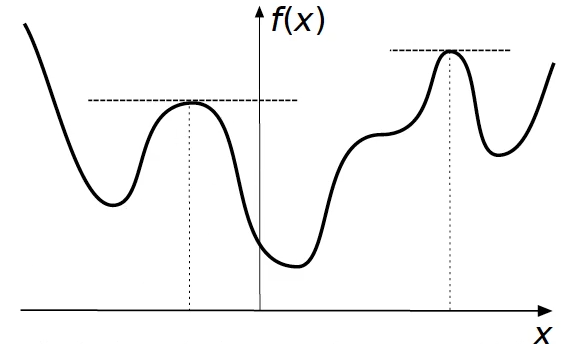
\includegraphics[scale=0.3]{figures/2/chapter2-towards_global1.png}
    \caption{Between a local minimum and a global minimum, there must be a local/global maximum.}
    \label{fig:chapter2-towards_global1}
\end{figure}
\par We want our function to have only local minimums in the stationary points. That is each time we are in a stationary point, we have a positive semi-definite matrix. In formula:
\begin{equation}
    \label{eq:sufficient-local-global}
    \nabla f(x) = 0 \Rightarrow \nabla^2 f(x) \succeq 0
\end{equation}
The sufficient condition for having \ref{eq:sufficient-local-global} is to have the positive semi-definite Hessian on the whole space over which our function is defined. That is:
\begin{equation}
    \forall x \in \mathbb{R}^n \dot \nabla^2 f(x) \succeq 0
\end{equation}
The functions satisfying this property are called \textbf{Convex Functions} (figure \ref{fig:chapter2-convex_function}).
\begin{figure}
    \centering
    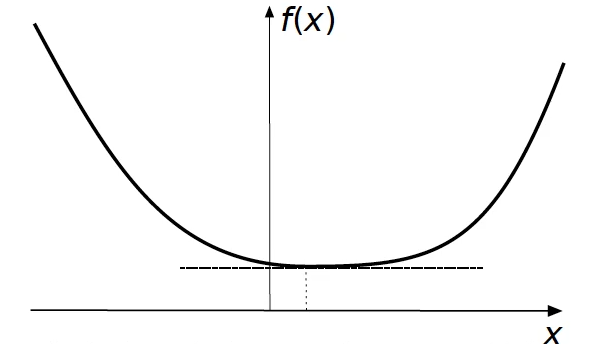
\includegraphics[scale=0.3]{figures/2/chapter2-convex_function.png}
    \caption{An example of a convex function.}
    \label{fig:chapter2-convex_function}
\end{figure}
\par Optimising convex functions is usually an easy problem (not always). Optimising non convex functions is instead a much more difficult problem. Infact in ML usually one always tries to build a convex model because every local minimum is also a global minimum, mathematically true. Whenever this is not possible, one usually does not require a global minimum and gets satisfied with a local one.
%
%
%
\section{Convexity}
\subsection{Introduction}
\par Given two points $x,y$ in a space $\mathbb{R}^n$, we define the segment (set of points) joining those two points with the following equation:
\begin{equation}
    \textit{conv}(x,y) = \{z = \alpha x + (1-\alpha) y \ :\ \alpha \in [0,1]\}
\end{equation}
\par Given a set, we say that it is a \textbf{convex set}, if any time we take two points inside the set, the segment joining these two points is entirely contained in the set (see figure \ref{fig:chapter2-convex_set}).
\begin{figure}
    \centering
    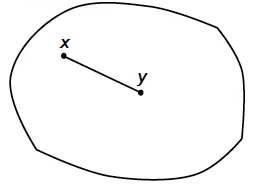
\includegraphics[scale=0.4]{figures/2/chapter2-convex_set.png}
    \caption{An example of the convex set with the segment joining two points entirely contained in the set.}
    \label{fig:chapter2-convex_set}
\end{figure}
Similarly, if the set does not contain the whole segment, the set is not a convex set (see figure \ref{fig:chapter2-non_convex_set}).
\begin{figure}
    \centering
    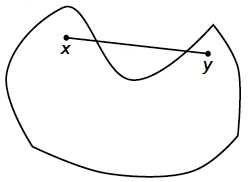
\includegraphics[scale=0.4]{figures/2/chapter2-non_convex_set.png}
    \caption{An example of the non convex set.}
    \label{fig:chapter2-non_convex_set}
\end{figure}
\par The nice thing is that every non convex set can be made a convex set. Basically, you perform a closure operation until there are some points to be added (see figure \ref{fig:chapter2-completed_non_convex_set}). There are actually in infinite number of sets that ``complete'' the non convex set, but the smallest one is of our interest and it is called \textbf{convex hull}.
\begin{figure}
    \centering
    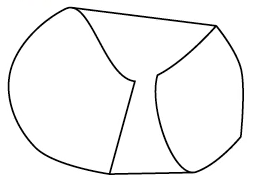
\includegraphics[scale=0.4]{figures/2/chapter2-completed_non_convex_set.png}
    \caption{Any non convex set can be completed into a convex set.}
    \label{fig:chapter2-completed_non_convex_set}
\end{figure}
\par Clearly, we can generalise the concept from above. Instead of using two points, we can use an arbitrarily large number of points.
\begin{equation}
    \textit{conv}(\{x_1,...,x_k\}) = \{x = \sum_{i=1}^k \alpha_i x_i\ :\ \sum_{i=1}^k \alpha_i = 1 \wedge \forall \alpha_i \geq 0\}
\end{equation}
\par We then have the following relation:
\begin{equation}
    C \textit{ is convex} \iff \textit{conv}(\{x_1,...,x_k\}) \subseteq C\  \forall x_1,...,x_k \in C
\end{equation}
In other words, a set $C$ is convex if every time we take $k$ elements and we make a convex hull of them, that convex hull is completely inside the $C$.
\par \textbf{Exercise}. Close and convex properties are not the same. Provide an example of a set that is closed but not convex and viceversa. Moreover, prove that:
\begin{equation}
    \label{eq:closed_and_convex}
    C \textit{ closed} \centernot \Rightarrow \textit{conv}(C) \textit{ closed}
\end{equation}
Ultimately, explain under which condition the logical equation \ref{eq:closed_and_convex} is true. Actually, quite always this is the case.
\par \textbf{Solution}. One example of a closed but not convex set is the set of natural numbers. An example of convex but not closed set is $(0,1)$. In order to prove \ref{eq:closed_and_convex}, we need an example of the closed set whose convex hull is not closed. TO FINISH.
%
\subsection{Examples of convex sets}
\par The convex sets are not rare. There are plenty of them, and we use some operations that preserve convexity in order to create other convex sets. Let us see some of the obvious convex sets:
\begin{itemize}
    \item Convex hull. Of course.
    \item Affine hyperplane: $\mathcal{H} = \{ax = b\ :\ x \in \mathbb{R}^n\}$. A hyperplane is a subspace whose dimension is one less than that of its ambient space. If a space is 3-dimensional then its hyperplanes are the 2-dimensional planes, while if the space is 2-dimensional, its hyperplanes are the 1-dimensional lines.
    \item Affine subspaces: $\mathcal{H} = \{ax \leq b\ :\ x \in \mathbb{R}^n\}$.
    \item Ball in $p$-norm, $p \geq 1$: $\mathcal{B}_p(x,r) = \{y \in \mathbb{R}^n\ :\ \Vert x-y \Vert_p \leq r\}$.
    \item Ellipsoid (figure \ref{fig:chapter2-ellipsoid}): $\mathcal{E}(Q,x,r) = \{y \in \mathbb{R}^n\ :\ (y-x)^T Q (y-x) \leq r\}$, and $Q$ positive semidefinite.
    \begin{figure}
        \centering
        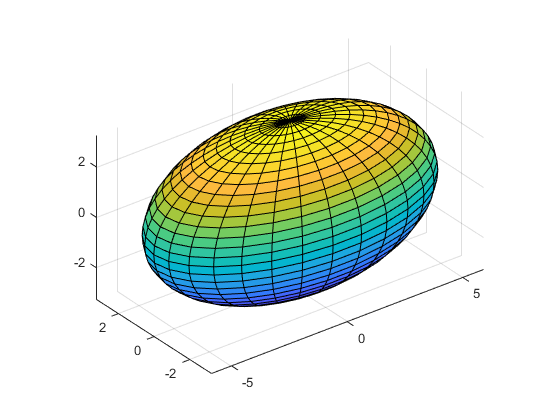
\includegraphics[scale=0.4]{figures/2/chapter2-ellipsoid.png}
        \caption{An example of an Ellipsoid.}
        \label{fig:chapter2-ellipsoid}
    \end{figure}
    \item All of the previous sets are closed, but also the open version is convex.
    \item Convex cones. There are different kinds of cones, for instances:
    \begin{itemize}
        \item Conical hull (polyhedral cone, see figure \ref{fig:chapter2-polyhedral_cone}):
        \begin{equation}
            \textit{cone}(\{d_1,...,d_k\}) = \{d = \sum_{i=1}^k \mu_i d_i\ :\ \mu_i \geq 0\ \forall i\}
        \end{equation}
        \begin{figure}
            \centering
            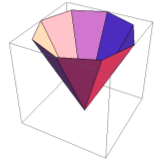
\includegraphics[scale=0.5]{figures/2/chapter2-polyhedral_cone.png}
            \caption{An example of a polyhedral cone.}
            \label{fig:chapter2-polyhedral_cone}
        \end{figure}
        \item Lorentz (ice-cream) cone (see figure \ref{fig:chapter2-lorentz_cone}):
        \begin{equation}
            \mathbb{L} = \Bigg\{x \in \mathbb{R}^n\ :\ x_n \geq \sqrt{\sum_{i=1}^{n-1} x_i^2}\Bigg\}
        \end{equation}
        \begin{figure}
            \centering
            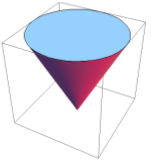
\includegraphics[scale=0.5]{figures/2/chapter2-lorentz_cone.png}
            \caption{An example of a Lorentz cone.}
            \label{fig:chapter2-lorentz_cone}
        \end{figure}
        \item Cone of the positive semidefinite matrices (see figure \ref{fig:chapter2-cones_positive_semidefinite_matrices}):
        \begin{equation}
            \mathbb{S}_+ = \{A \in \mathbb{R}^{n \times n}\ :\ A \succeq 0\}
        \end{equation}
        \begin{figure}
            \centering
            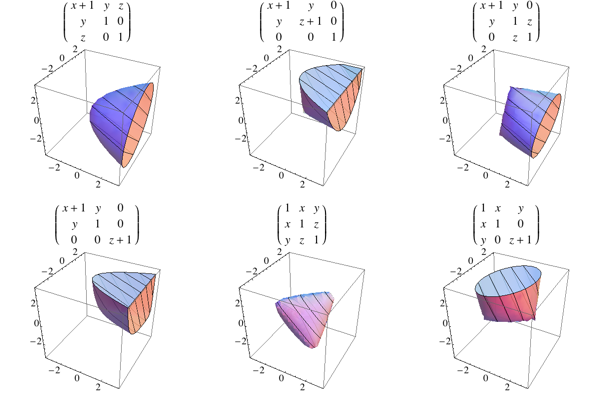
\includegraphics[scale=0.4]{figures/2/chapter2-cones_positive_semidefinite_matrices.png}
            \caption{Some examples of positive semidefinite matrices that generate cones.}
            \label{fig:chapter2-cones_positive_semidefinite_matrices}
        \end{figure}
        The last two cases of cones, are examples of non-polyhedral cones.
    \end{itemize}
\end{itemize}
\par \textbf{Exercise}. Prove that the above sets are convex. Provide an example of a non convex cone.
%
\subsection{Operations that preserve convexity}
\par Let us now see some operations that preserve the convexity. These operations are frequently used to extend the set of convex sets.
\begin{itemize}
    \item The intersection of convex sets $\{C_i\}_{i \in I} = \bigcap_{i \in I} C_i$ is a convex set.
    \item The Cartesian product of convex sets $\{C_i\}_{i \in I} = C_1 \times ... \times C_{|I|}$ is a convex set.
    \item Given a convex set $C$, then the image of its linear transformation (scaling, rotating, translating) $A(C) = \{x = Ay + b\ :\ y \in C\}$ is a convex set.
    \item Given a convex set $C$, then the inverse image of its linear transformation (scaling, rotating, translating) $A^{-1}(C) = \{x\ :\ Ax + b \in C\}$ is a convex set.
    \item Given two convex sets $C_1$ and $C_2$, then its linear combination $\alpha_1 C_1 + \alpha_2 C_2 = \{x = \alpha_1 x_1 + \alpha_2 x_2\ :\ x_1 \in C_1, x_2 \in C_2\}$ with any $\alpha_1, \alpha \in \mathbb{R}$ is a convex set.
    \item Slice is a convex set: given that $C \subseteq \mathbb{R}^n = \mathbb{R}^{n_1} \times \mathbb{R}^{n_1}$, then we define slice $C(y) = \{x \in \mathbb{R}^{n_1}\ :\ (x,y) \in C\}$ (see figure \ref{fig:chapter2-slice}).
    \begin{figure}
        \centering
        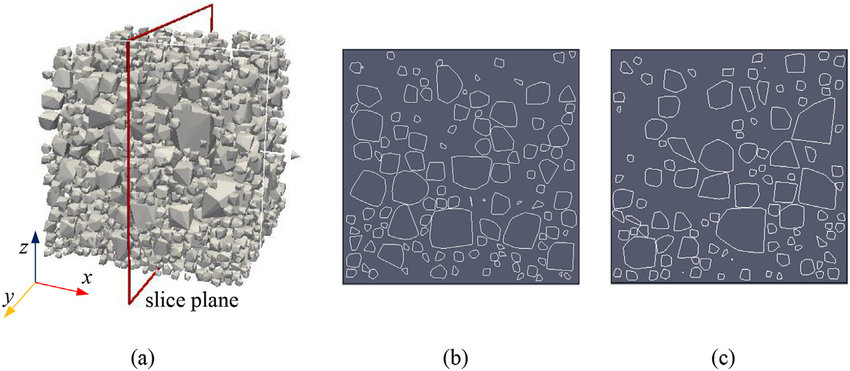
\includegraphics[scale=0.3]{figures/2/chapter2-slice.png}
        \caption{An example of a slice object.}
        \label{fig:chapter2-slice}
    \end{figure}
    \item Shadow is a convex set: given that $C \subseteq \mathbb{R}^n = \mathbb{R}^{n_1} \times \mathbb{R}^{n_1}$, then we define shadow $C^1 = \{x \in \mathbb{R}^{n_1}\ :\ \exists y\ s.t.\ (x,y) \in C\}$ (see figure \ref{fig:chapter2-shadow}).
    \begin{figure}
        \centering
        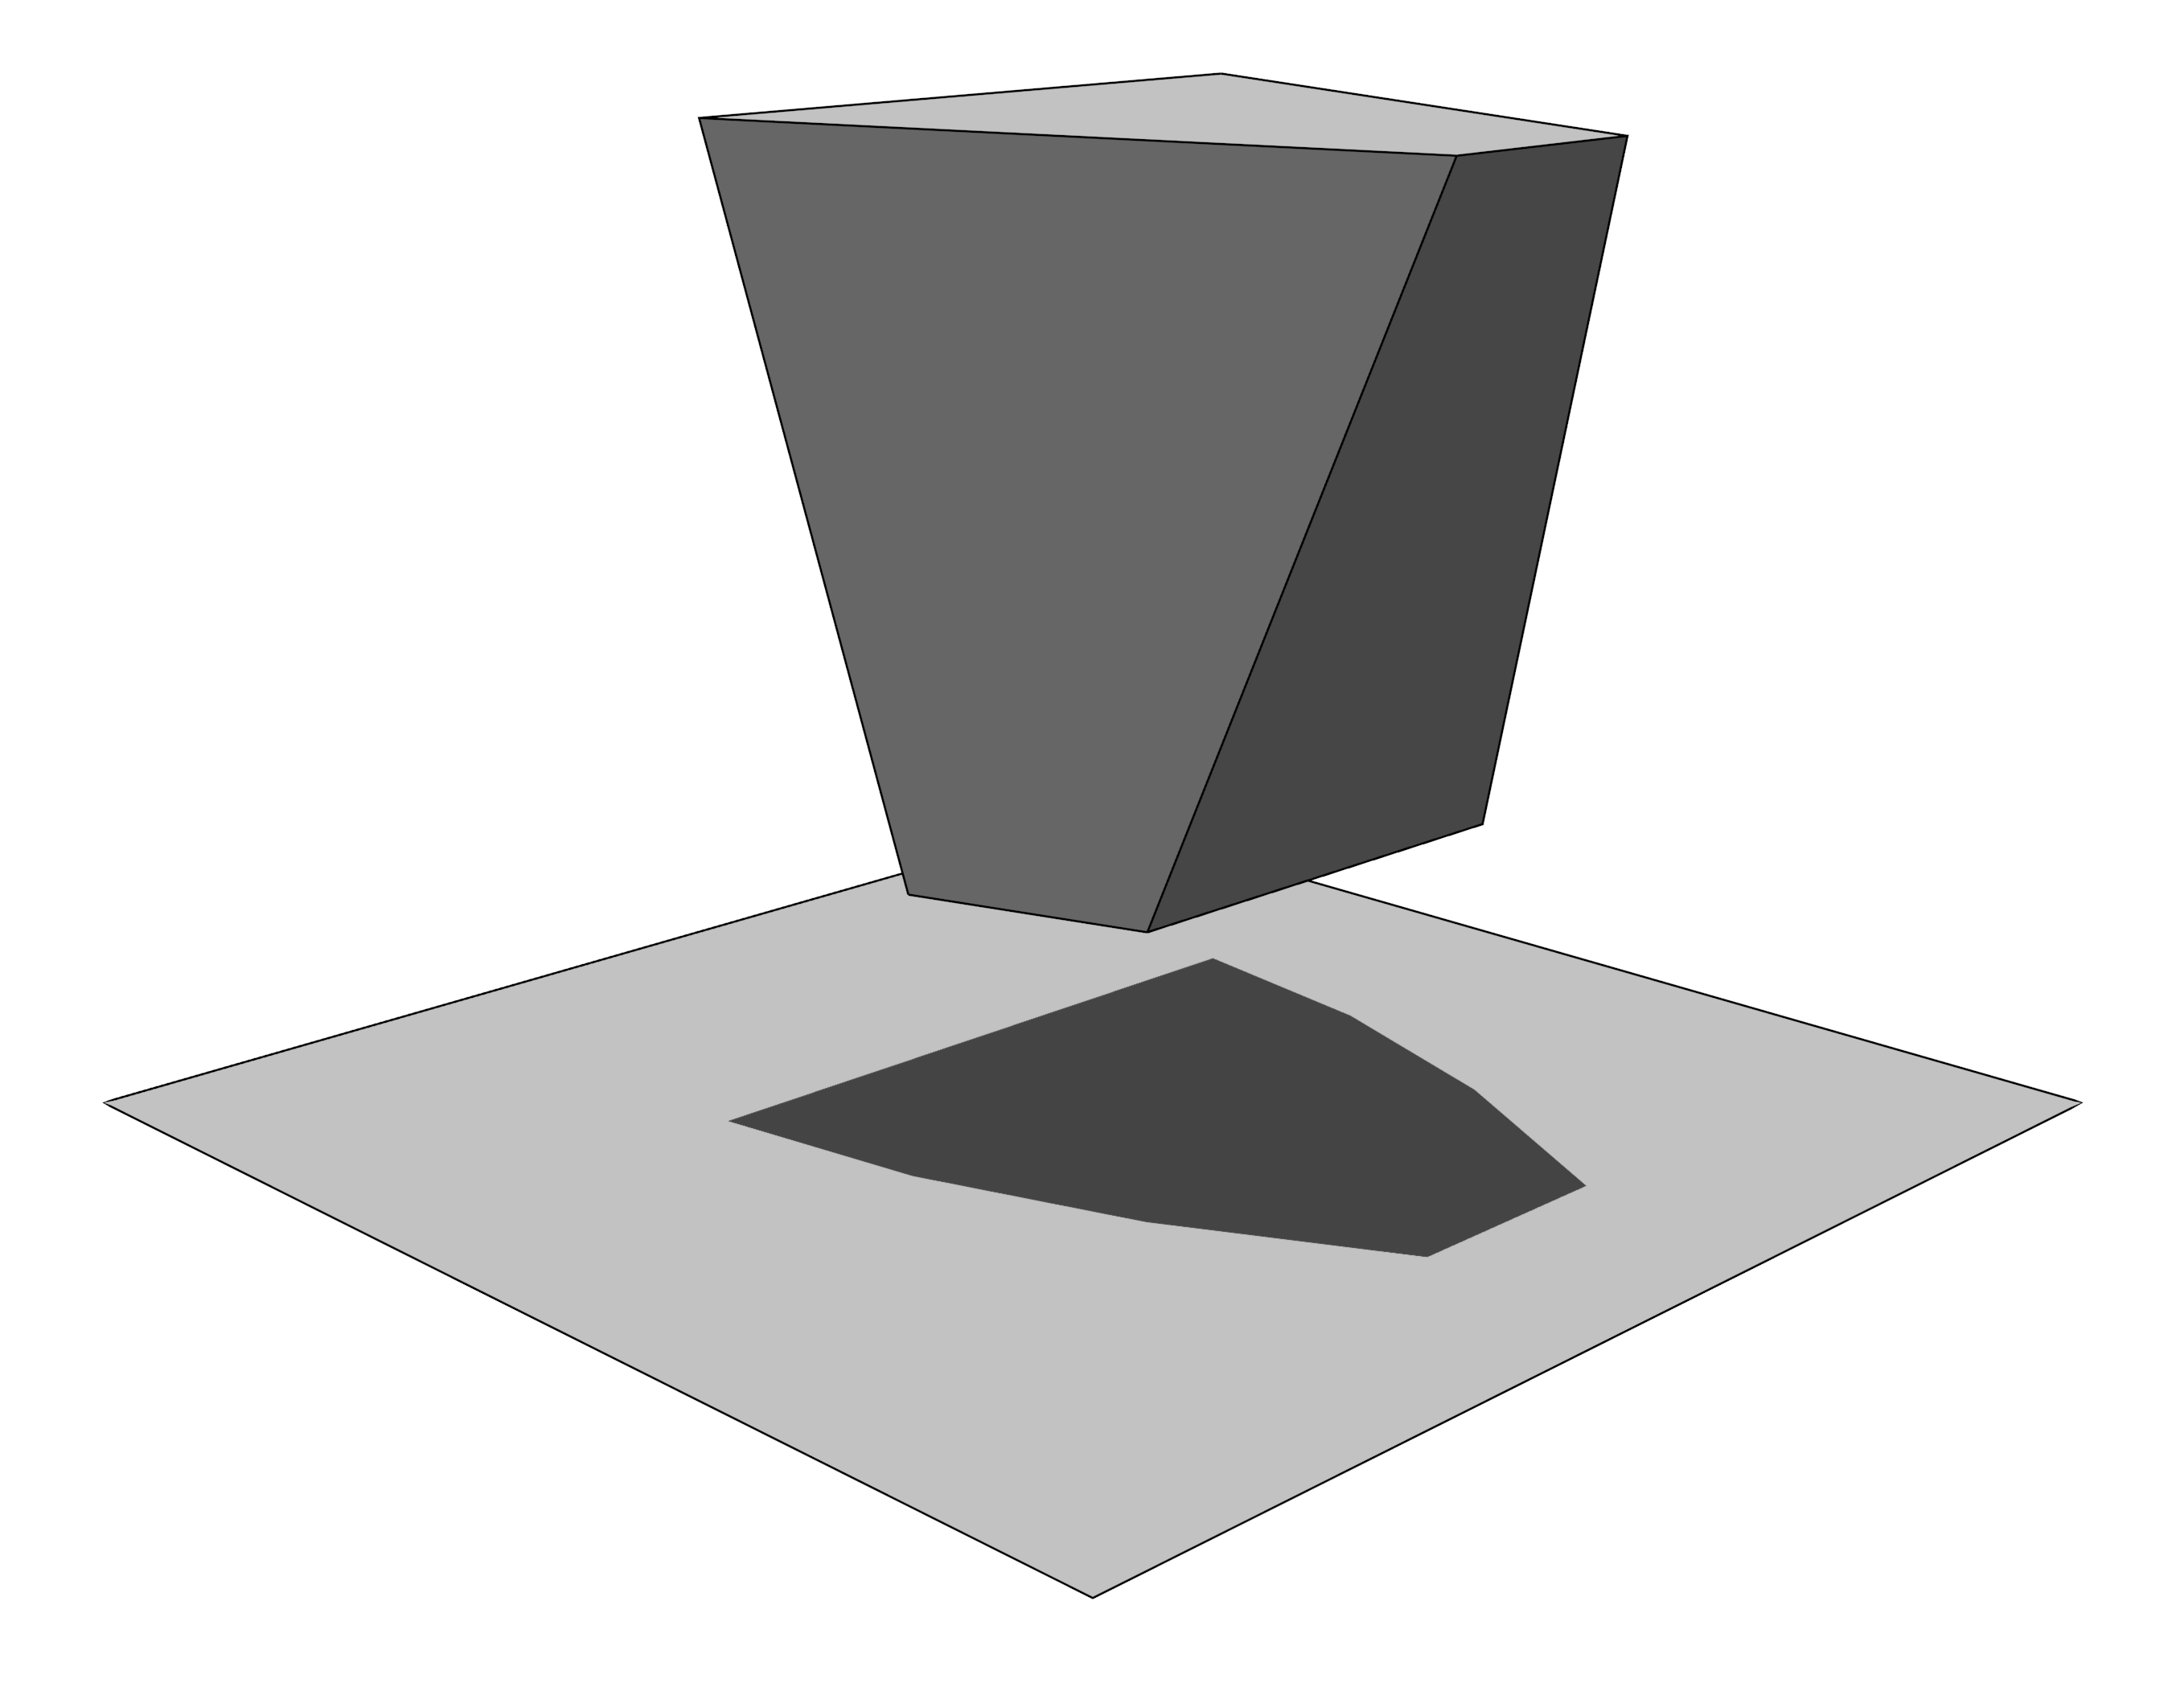
\includegraphics[scale=0.05]{figures/2/chapter2-shadow.png}
        \caption{An example of a shadow object.}
        \label{fig:chapter2-shadow}
    \end{figure}
\end{itemize}
\par \textbf{Exercise}. Is the union of two convex set convex? Given a matrix $A \in \mathbb{R}^{m \times n}$, prove that the polyhedron of type $\mathcal{P} = \{x \in \mathbb{R}^n\ :\ Ax \leq b\}$ is convex.
\par \textbf{Exercise}. Given a polyhedron $\mathcal{P}$, prove that $\{d\ :\ x + \alpha d \in \mathcal{P}, \forall x \in \mathcal{P}, \alpha \geq 0\}$ (its recession cone) is a cone. (hint: look at $\mathcal{C} = \{x \in \mathbb{R}^n\ :\ Ax \leq 0\}$)
%
\subsection{Convex functions}
\par Let us define a convex function informally. A function is said to be convex if for any two points of its domain, the line connecting those two points is completely above the function itself (see figure \ref{fig:chapter2-informal_convex_function}).
\begin{figure}
    \centering
    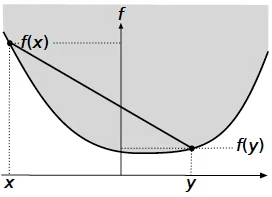
\includegraphics[scale=0.6]{figures/2/chapter2-informal_convex_function.png}
    \caption{An example of a convex function.}
    \label{fig:chapter2-informal_convex_function}
\end{figure}
\par Formally (see figure \ref{fig:chapter2-formal_convex_function}), for any two points $x,y \in \text{dom}(f) \subseteq \mathcal{R}^n, \alpha \in [0,1]$ we have that:
\begin{equation}
    \alpha f(x) + (1-\alpha)f(y) \geq f(\alpha x + (1-\alpha)y)
\end{equation}
What we are saying is that given two points in the domain of the function, the line connecting them is the approximation model of the real function, given that we know just those two points. This line is at least the very same piece of the function $f$ or it must be that it is above. This must happen for every two points in the domain of $f$ in order to define $f$ convex.
\begin{figure}
    \centering
    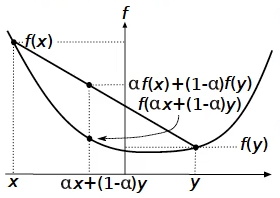
\includegraphics[scale=0.6]{figures/2/chapter2-formal_convex_function.png}
    \caption{The definition of the convex function.}
    \label{fig:chapter2-formal_convex_function}
\end{figure}
\par Let us now be a little bit more Einstein and generalise the above convex definition to more than two points.
\begin{equation}
    \forall x_1,...,x_k, \forall \alpha_1,...,\alpha_k \in [0,1]\ s.t.\ \sum_{i=1}^k \alpha_i = 1\ .\ f\Big(\sum_{i=1}^k \alpha_i x_i\Big) \leq \sum_{i=1}^k \alpha_i f(x_i)
\end{equation}
\par \textbf{Property}. If a function $f$ is convex, then any level set $S(f,v)$ is convex $\forall v \in \mathbb{R}$. TODO proof.
\par Nevertheless, it is not true the reverse. It is not true that if $\forall v \in \mathbb{R}$ level set $S(f,v)$ is convex then $f$ is itself convex. Counterexample? Imagine Bullet-nose curve in some dimension. Yeah, you said: err.. imagine what?? See the figure \ref{fig:chapter2-sandglass}. Clearly whatever level set has to be convex. But, this is not a convex function.
\begin{figure}
    \centering
    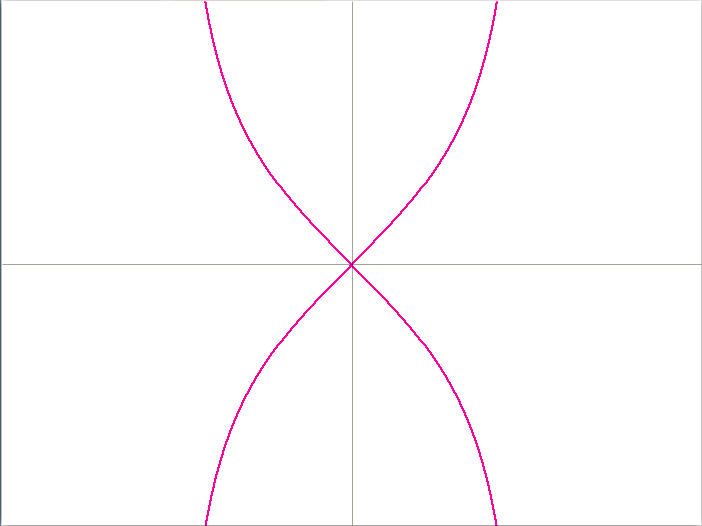
\includegraphics[scale=0.3]{figures/2/chapter2-sandglass.png}
    \caption{Bullet-nose curve. Also called sandglass by humans.}
    \label{fig:chapter2-sandglass}
\end{figure}
\par There is also a strict version of the convexity, where the signs $\leq,\geq$ are exchanged with their strict alternative, i.e. $<,>$.
\par One particularly important version of convexity is \textbf{strong convexity}. $f$ is said to be strongly convex with modulus $\tau > 0$ if the following holds:
\begin{equation}
    f(x)-\frac{\tau}{2}\Vert x \Vert^2
\end{equation}
or in more obvious terms:
\begin{equation}
    \alpha f(x) + (1-\alpha) f(y) \geq f(\alpha x + (1-\alpha) y) + \frac{\tau}{2} \alpha(1-\alpha) \Vert x-y \Vert^2
\end{equation}
This basically means that the functions is bellow quadratically much. In other words, given a point $x$ our function $f$ in that point is steeper than the quadratic model in that point.
\par Convex functions cannot be unbounded bellow. The only case of a convex function that is unbounded below is the linear case, in any dimension.
\par Last but not least, $f$ is called concave if $-f$ is convex. Clearly, we have also strictly and strongly concave functions.
%
\subsection{Prototypical convex functions}
\par As for the convex sets, we have some prototypical functions that are simple and we know that are convex. These, and many other, functions can be composed to get more complicated convex functions.
\par Let us illustrate some of the simplest convex functions:
\begin{itemize}
    \item $f(x) = wx$, i.e. the linear object. This is the only case that is both convex and concave.
    \item $f(x) = \frac{1}{2}x^T Q x + qx$ quadratic function, convex if and only if the Hessian matrix is positive semidefinite.
    \item $f(x) = e^{\alpha x}, \forall \alpha \in \mathbb{R}, x \in \mathbb{R}^n$ the exponential function.
    \item $f(x) = - \log(x), x > 0$ the complement logarithm function.
    \item $f(x) = x^\alpha, \forall \alpha \in \mathbb{R} \setminus (0,1), x \in \mathbb{R}^n$ the power function.
    \item $f(x) = \Vert x \Vert_p, p \geq 1$ the norm function.
    \item $f(x) = \max\{x_1,...,x_n\}$ the maximum function.
    \item For any convex set $C$, its indicator function is convex:
    \begin{equation}
        I_C(x) = \begin{cases} 0, & \mbox{if } x \in C \\ +\infty, & \mbox{if } x \notin C \end{cases}
    \end{equation}
    The indicator function simply maps to 0 all the elements that belong to the set and to +$\infty$ those that don't. Since the underlying set is convex, it is obvious that the mathematical object that we obtain when we apply the indicator function transformation is indeed convex.
\end{itemize}
\par \textbf{Exercise}. Prove that the above functions are convex.
\par \textbf{Exercise}. Is the function $f(x) = \min\{x_1,...,x_n\}$ convex?
\subsection{Functional operations that preserve convexity}
\par Let us now show some of the composition operators that can be used over convex functions in order to get other, more complex, convex functions. There are basically two ways of checking if a given function $f$ is convex. Either we compute the Hessian and then verify that it is positive semidefinite everywhere on the function domain, or we try to get $f$ as composition of some basic convex functions using the some operators that preserve convexity. Some of these operators are:
\begin{itemize}
    \item Given $f$ and $g$ convex, $\alpha, \beta \in \mathbb{R}_+$, then the linear non negative combination $\alpha f + \beta g$ is also convex.
    \item Given a set of infinitely many convex functions $\{f_i\}_{i \in I}$, the function $f(x) = \sup_{i \in I} f_i(x)$ is convex.
    \item Given a convex function $f$, then the linear precomposition $f(Ax+b)$ is also convex.
    \item Given a convex multivariable function $f : \mathbb{R}^n \rightarrow \mathbb{R}$ and a convex increasing function $g : \mathbb{R} \rightarrow \mathbb{R}$, the composition $g \circ f = g(f(x))$ is a convex function.
    \item FINISH THE REMAINING
\end{itemize}
\par \textbf{Exercise}. Prove that the above composition operators preserve the convexity.
%
\subsection{First order conditions over convex functions}
\par The question is: why the heck we like the convex functions so much? Are they that pretty? Yes. They are like Sweden girls.
\par Given a function $f$ that is convex, then its gradient exists almost everywhere. Let us prove the following property:
\begin{equation}
    f \in C^1 \mbox{convex over convex set C} \iff f(y) \geq f(x) + (y-x)\nabla f(x), \forall x,y \in C
    \label{eq:chapter2-first_order_convex}
\end{equation}
In other words, the linear model of our function $f$ tangent in the point $x$ is always under the function in whatever other point $y$ (see figure \ref{fig:chapter2-first_order_convex}).
\begin{figure}
    \centering
    \begin{subfigure}{0.31\textwidth}
    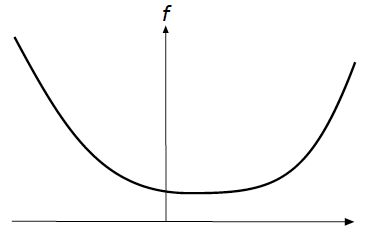
\includegraphics[width=\linewidth]{figures/2/first-order-convex/1.png}
    \caption{Suppose you have a convex function} \label{fig:foc1}
    \end{subfigure}
    \begin{subfigure}{0.31\textwidth}
    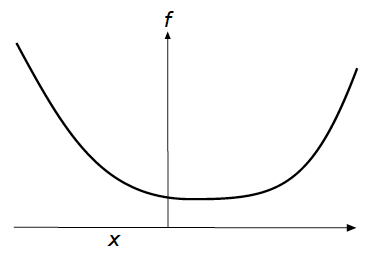
\includegraphics[width=\linewidth]{figures/2/first-order-convex/2.png}
    \caption{Take a point $x$} \label{fig:foc2}
    \end{subfigure}
    \begin{subfigure}{0.31\textwidth}
    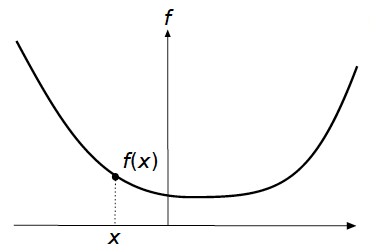
\includegraphics[width=\linewidth]{figures/2/first-order-convex/3.png}
    \caption{Project on $f$ and take its value} \label{fig:foc3}
    \end{subfigure}
    \begin{subfigure}{0.31\textwidth}
    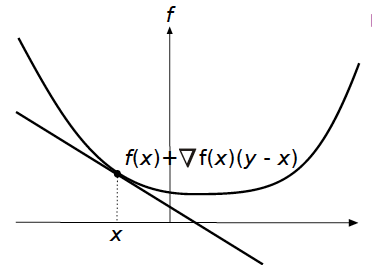
\includegraphics[width=\linewidth]{figures/2/first-order-convex/4.png}
    \caption{Build the linear model in point $x$. Call it $L_x$} \label{fig:foc4}
    \end{subfigure}
    \hspace*{\fill} % separation between the subfigures
    \begin{subfigure}{0.31\textwidth}
    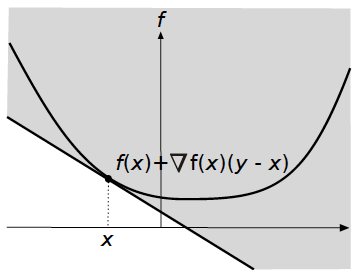
\includegraphics[width=\linewidth]{figures/2/first-order-convex/5.png}
    \caption{The epigraph of $L_x$} \label{fig:foc5}
    \end{subfigure}
    \hspace*{\fill} % separation between the subfigures
    \begin{subfigure}{0.31\textwidth}
    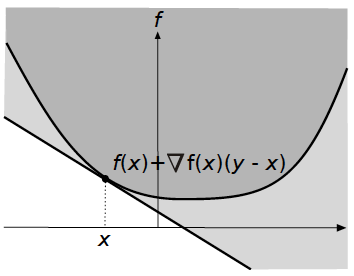
\includegraphics[width=\linewidth]{figures/2/first-order-convex/6.png}
    \caption{The epigraph of $f$, subset of the epigraph of $L_x$} \label{fig:foc6}
    \end{subfigure}
    \caption{Visual explanation of the equation \ref{eq:chapter2-first_order_convex}.}
    \label{fig:chapter2-first_order_convex}
\end{figure}
\par What happens when we have the gradient 0? That is, what happens if we are in a stationary point? Well, the following happens (see figure \ref{fig:chapter2-first_order_convex_stationary}):
\begin{equation}
    \nabla f(x) = 0 \Rightarrow f(y) \geq f(x), \forall y \in \mathbb{R}^n
    \label{eq:chapter2-first_order_convex_stationary}
\end{equation}
\begin{figure}
    \centering
    \begin{subfigure}{0.31\textwidth}
    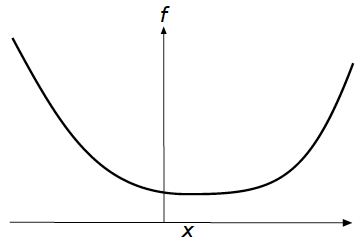
\includegraphics[width=\linewidth]{figures/2/first-order-convex/7.png}
    \caption{Point $x$ is a stationary point} \label{fig:foc7}
    \end{subfigure}
    \begin{subfigure}{0.31\textwidth}
    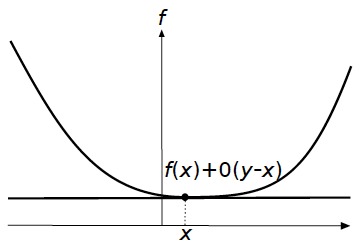
\includegraphics[width=\linewidth]{figures/2/first-order-convex/8.png}
    \caption{$\nabla f(x) = 0$} \label{fig:foc8}
    \end{subfigure}
    \begin{subfigure}{0.31\textwidth}
    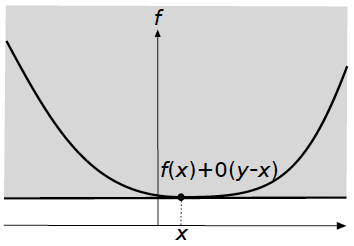
\includegraphics[width=\linewidth]{figures/2/first-order-convex/9.png}
    \caption{Epigraph of $L_x$} \label{fig:foc9}
    \end{subfigure}
    \begin{subfigure}{0.31\textwidth}
    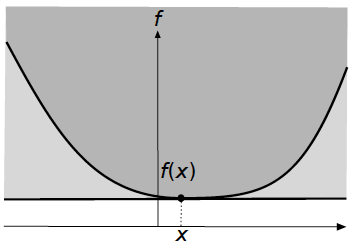
\includegraphics[width=\linewidth]{figures/2/first-order-convex/91.png}
    \caption{Epigraph of $f(x)$} \label{fig:foc91}
    \end{subfigure}
    \caption{Visual explanation of the equation \ref{eq:chapter2-first_order_convex_stationary}.}
    \label{fig:chapter2-first_order_convex_stationary}
\end{figure}
\par What?! Yes, exactly! If we are in a stationary point $x$, pick any other $y$ from the function domain, the value of $f$ in $y$ will be $\geq$ than the value in the point $x$. Wait, but that means that...? Yes! That means that $x$ is the global minimum solution and that $f(x)$ is the global minimum value. That's!, why the heck we like the convex functions!
\begin{theorem}
    Given $f$ convex and continuous, then if $x$ is a stationary point of $f$ then $x$ is the global minimum.
\end{theorem}
%
\subsection{Second order conditions over convex functions}
\par We said that proving that the function is convex entirely on its domain requires computing its Hessian. In order to be able to do that we need the function to be continuously differentiable, that is it needs to have continuous first derivative. Usually, this is the simplest way to check convexity of a function.
\begin{theorem}
    A function $f \in C^2$, i.e. continuously differentiable, is convex over an open domain $S$ if and only if its Hessian is positive semidefinite, in formulae:
    \begin{equation}
        f \mbox{ is convex} \iff \nabla^2 f(x) \succeq 0
    \end{equation}
\end{theorem}
\par TODO add exercises from the slide
%
\subsection{Subgradients and subdifferentiales}
\par Convexity is nice. But we spoke only about differentiable stuff, otherwise no gradient and no Hessian. Do we really need differentiability? Well, no. With convex functions we can even non differentiable things. But it get complicated.
\par As a side note, consider the function $f$ and the set over which is defined to be convex. We could actually define the minimisation problem in the following way:
\begin{equation}
    (P) \equiv \inf\{f_X(x) = f(x) + I_X(x) : x \in \mathbb{R}^n\}
\end{equation}
Where $I_X(x)$ is the indicator function, which is non differential by design. $f_X$ is called \textbf{essential objective}. Now look at this magic:
\begin{equation}
    x_* \mbox{ is a global optimum} \iff x_* \mbox{ is local minimum for } f_X
\end{equation}
\begin{proof}
    By contradiction. Assume $\exists y \in \mathbb{R}^n : f(y) < f(x_*)$. Then:
    \[
        f(x_*) \leq f(\alpha x_* + (1-\alpha) y) \leq \alpha f(x_*) + (1 - \alpha) f(y) < f(x_*)
    \]
    Which is a contradiction.
\end{proof}
\par Cool. But the question is still: how do I identify the local minimum without the gradient $\nabla f(x)$? We don't have the gradient. We need something that is similar to the gradient but not the gradient :). What was the main property of the gradient when we looked at first order conditions? The epigraph. Consider again something like in figure \ref{fig:chapter2-foc9}. The important thing was that the epigraph of the linear model was under the epigraph of the actual function it was approximating in the stationary point. In other point, it is not important that it is the gradient but that it is completely under the function.
\begin{figure}
    \centering
    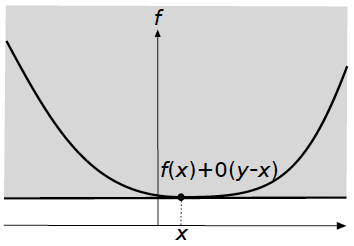
\includegraphics[scale=0.4]{figures/2/first-order-convex/9.png}
    \caption{Caption}
    \label{fig:chapter2-foc9}
\end{figure}
\par So what is the subgradient $s$ of $f$, the country cousin of the gradient $\nabla$:
\begin{equation}
    s \mbox{ is the subgradient of } f \mbox{ in } x \iff f(y) \geq f(x) + s(y-x), \forall y \in \mathbb{R}^n
    \label{eq:subgradient}
\end{equation}
\par Consider the function in figure \ref{fig:sub_diffs1}. As you can see, there are some kinks. One of the kinks is also our nice global minimum (figure \ref{fig:sub_diffs2}). In those kinks there are infinitely many linear models that satisfy the equation \ref{eq:subgradient} (see figure \ref{fig:sub_diffs3}). And that is fine. Because in that point we can have a (sub)gradient that is 0.
\begin{figure}
    \centering
    \begin{subfigure}{0.31\textwidth}
        \centering
        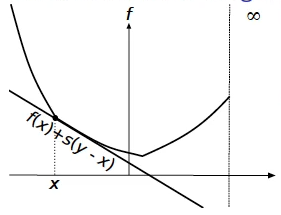
\includegraphics[scale=0.4]{figures/2/sub-diffs/sub_diffs1.png}
        \caption{Caption}
        \label{fig:sub_diffs1}
    \end{subfigure}
    \begin{subfigure}{0.31\textwidth}
        \centering
        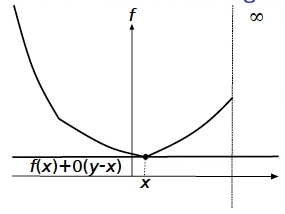
\includegraphics[scale=0.4]{figures/2/sub-diffs/sub_diffs2.png}
        \caption{Caption}
        \label{fig:sub_diffs2}
    \end{subfigure}
    \begin{subfigure}{0.31\textwidth}
        \centering
        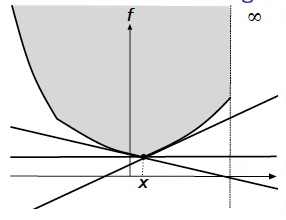
\includegraphics[scale=0.4]{figures/2/sub-diffs/sub_diffs3.png}
        \caption{Caption}
        \label{fig:sub_diffs3}
    \end{subfigure}
\end{figure}
\par What is the problem? The problem is that in the point that is actually a stationary point, and so the gradient is 0, and so it is a local minimum, and so due to the convexity it is also a global minimum; there are infinitely many subgradients. A sub set of these tell you go on the right to find the minimum, another set tells you go on the left, and a singleton set tells you that you are at the right place. Solutions? Keep a set of subgradients.
\par Let us now define the \textbf{subdifferential}:
\begin{equation}
    \partial f(x) = \{s \in \mathbb{R}^n : s \mbox{ is a subgradient at } x\}
\end{equation}
\par Clearly, if $f$ is differentiable in $x$ then it must be the case that the subdifferential is a singleton set containing just the regular gradient.
\par You remember that the gradient characterise all the directional derivatives in a point $x$ (scalar product). If you want to know if a direction is a descent direction, you just need to compute the scalar product with the directional derivative and the gradient. It turns out that with subgradient it is a bit more complicated. Taking just one gradient does not tells you the whole story. If you want to be sure that you are going in the descent direction, you need to have a subdifferential full of directions that in scalar product with the gradient give a negative value.
\par The steepest descent direction for such non differentiable functions in a point of a kink, the computation requires solving an optimisation problem:
\begin{equation}
    s_* = - \mbox{argmin}\{\Vert s \Vert : s \in \partial f(x)\}
\end{equation}
Note that the set over which this problem is operating, i.e. subdifferential, is closed and convex. Thus it is again a convex optimisation. Note also that if the solution is 0, it means that we are in the global minimum.
\par Let us now consider the following example. In figure \ref{fig:sub_example1} you can see the level sets of the multivariable function:
\begin{equation}
    f(x,y) = \max\{x^2 + (y-1)^2, x^2 + (y+1)^2\}
\end{equation}
This function is convex, non differentiable, and the minimum value is located in the point $x_* = [0,0]$.
\par In the differentiable case the things are easy (figure \ref{fig:sub_example2}), we have our nice gradient that is normal (orthogonal) to the level sets and the opposite of it goes straight to the minimum (figure \ref{fig:sub_example3}), the steepest descent direction. Actually, whatever direction that is opposite to the gradient is a descent direction (figure \ref{fig:sub_example4}).
\par This does not occur in the non differentiable points. Suppose you are in the point shown on figure \ref{fig:sub_example5}. In that case, we have infinitely many subgradients. In particular, there are two directions (one is shown in figure \ref{fig:sub_example6}), that are not even pointing in the direction of the descent (they are pointing out of the level set). In other words, in those two directions the function is increasing. Nevertheless, the two direction form a closed and convex set that you can see in figure \ref{fig:sub_example7}. Each of the direction in that set is obtainable from the convex combination of these two extreme directions. The point is that each of these directions points inside the level set (figure \ref{fig:sub_example8}) and the one with the smallest norm is actually the steepest descent direction (figure \ref{fig:sub_example9}).
\begin{figure}
    \centering
    \begin{subfigure}{0.31\textwidth}
        \centering
        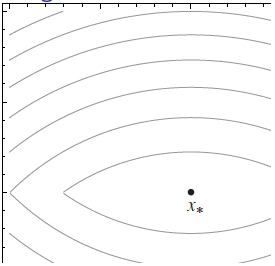
\includegraphics[scale=0.35]{figures/2/sub-example/sub_example1.png}
        \caption{Caption}
        \label{fig:sub_example1}
    \end{subfigure}
    \begin{subfigure}{0.31\textwidth}
        \centering
        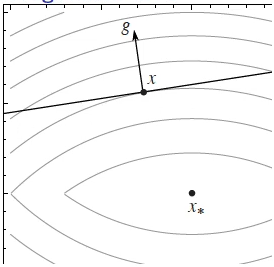
\includegraphics[scale=0.35]{figures/2/sub-example/sub_example2.png}
        \caption{Caption}
        \label{fig:sub_example2}
    \end{subfigure}
    \begin{subfigure}{0.31\textwidth}
        \centering
        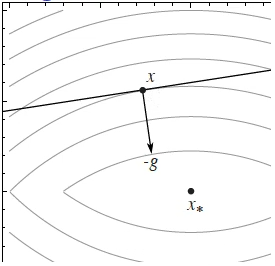
\includegraphics[scale=0.35]{figures/2/sub-example/sub_example3.png}
        \caption{Caption}
        \label{fig:sub_example3}
    \end{subfigure}
    \begin{subfigure}{0.31\textwidth}
        \centering
        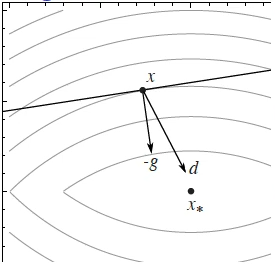
\includegraphics[scale=0.35]{figures/2/sub-example/sub_example4.png}
        \caption{Caption}
        \label{fig:sub_example4}
    \end{subfigure}
    \begin{subfigure}{0.31\textwidth}
        \centering
        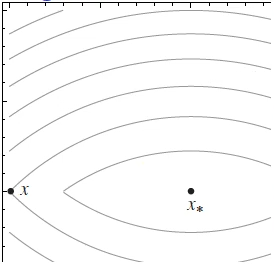
\includegraphics[scale=0.35]{figures/2/sub-example/sub_example5.png}
        \caption{Caption}
        \label{fig:sub_example5}
    \end{subfigure}
    \begin{subfigure}{0.31\textwidth}
        \centering
        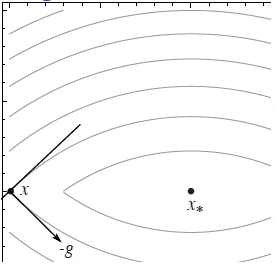
\includegraphics[scale=0.35]{figures/2/sub-example/sub_example6.png}
        \caption{Caption}
        \label{fig:sub_example6}
    \end{subfigure}
    \begin{subfigure}{0.31\textwidth}
        \centering
        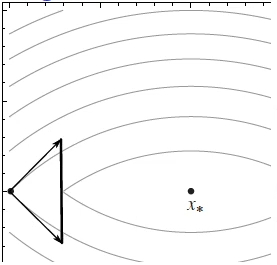
\includegraphics[scale=0.35]{figures/2/sub-example/sub_example7.png}
        \caption{Caption}
        \label{fig:sub_example7}
    \end{subfigure}
    \begin{subfigure}{0.31\textwidth}
        \centering
        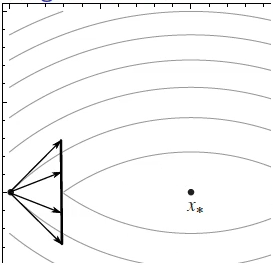
\includegraphics[scale=0.35]{figures/2/sub-example/sub_example8.png}
        \caption{Caption}
        \label{fig:sub_example8}
    \end{subfigure}
    \begin{subfigure}{0.31\textwidth}
        \centering
        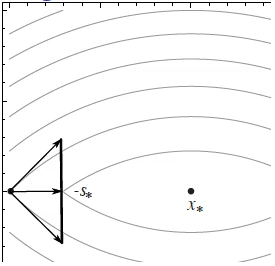
\includegraphics[scale=0.35]{figures/2/sub-example/sub_example9.png}
        \caption{Caption}
        \label{fig:sub_example9}
    \end{subfigure}
\end{figure}
%
\subsection{Subdifferential calculus}
\par Like in the case of convex sets and convex functions composition operators that preserve convexity, we have similarly the composition operations over subdifferentials that preserve subdifferentiability.
\par Let us now illustrate some of these composition operators:
\begin{itemize}
    \item TODO
\end{itemize}
%
\subsection{Approximate subgradients}
\par TODO
%
%
%
\section{Descent Methods}
\par Let us now ask our self a very basic question: what is so special with the gradient? Can we use something different? The answer is yes. The only thing that we really care about is to go in a \textit{descent} direction. The crucial arguments in our previous proofs about convergence was that the derivative was promising a significant descent along the direction $d = -\nabla f(x)$. But what if our direction is, let's say, rotated 45 degrees? We would still go in a descent direction. So we would expect the various proofs to carry on even in these cases, provided that the angle with the opposite of the gradient and the descent direction is not too big.
\par Let us now define mathematically a descent direction. A \textbf{descent direction} is a direction $d$ such that:
\begin{equation}
    d = \frac{\partial f}{\partial d^i}(x^i) \equiv d \cdot \nabla f(x) < 0 \equiv \cos (\theta^i) \geq 0
\end{equation}
This means that the direction $d$ points roughly in the same direction of $-\nabla f(x^i)$.
\par There are infinitely many descent direction of course. The whole half space of descent directions. There is a nice result called \textit{Zoutendijk condition} that states the following:
\begin{theorem}
    Suppose we have a bounded function whose gradient is Lipschitz continuous. Then under Armijo and strong Wolfe we have that:
    \begin{equation}
        \sum_{i=1}^\infty \cos^2(\theta^i)\Vert \nabla f(x^i) \Vert^2 < \infty
    \end{equation}
\end{theorem}
Basically, this means that provided that the angle $\theta^i$ between $-\nabla f(x^i)$ and $d^i$ is not too big, our sequence is converging to the minimum, i.e. $\nabla f(x)$ converges to 0. Think of the sequence that instead of moving straight to the minimum (when $d^i = -\nabla f(x^i)$), it circulate around in a spiral manner, until it reaches the minimum (centre). This happens provided that the angle is not too big. Actually Zoutendijk says that the sequence converges also in case $\theta^i$ converges to 90 degrees with the gradient ($\cos (\theta^i)$ converges to 0) provided that it does not converge too fast.
\par Note that if $\cos^2(\theta^i) = 1$ the formula above is the usual gradient method.
\par Note also that usually a non negative sequence has to converge to 0 quite fast in order for the summation to be convergent. Here, on the contrary, we require the sequence to not converge to 0 that fast, in order to have the overall summation convergent.
%
%
%
\section{Newton Method}
\par Let us now talk about one of the most important methods for unconstrained optimisation, the \textbf{Newton method}. You want a better direction? Use a better model. So instead of using just linear approximation, use the quadratic one.
\par Let us assume that the Hessian is positive definite:
\begin{equation}
    \nabla^2 f(x) \succ 0
\end{equation}
So our second order model becomes:
\begin{equation}
    f(x^i) + \nabla f(x^i) (x - x^i) + \frac{1}{2} \nabla^2 f(x^i) (x - x^i)
\end{equation}
A side note: it is easy to say ``let us use the Hessian''. But suppose you have a function of thousands of variables. Since Hessian is a square matrix, its dimensions are order of millions. Those are huge matrices to deal with.
\par The Newton direction $d^i$ is defined as:
\begin{equation}
    d^i = - [\nabla^2 f(x^i)]^{-1} \nabla f(x^i)
\end{equation}
Remember that in order to Newton to work, the quadratic model has to have a minimum. This basically means that the Hessian needs to be positive semi definite. But since in the direction computation we also need it invertible (non singular) we must require that the matrix is positive definite.
\par Consider the following nonlinear equation interpretation of Newton method. What we want to do is to solve the nonlinear set of equations of the form $\nabla f(x) = 0$. What we can do is to ``linearise'' this nonlinear system by applying Taylor to the gradient:
\begin{equation}
    \nabla f(x) \approx \nabla f(x^i) + \nabla^2 f(x^i) (x - x^i)
\end{equation}
Since we are looking for $\nabla f(x) = 0$ the model becomes:
\begin{equation}
    (x - x^i) \approx - [\nabla^2 f(x^i]^{-1} \nabla f(x) 
\end{equation}
And what is $x - x^i$? It is the direction from the point $x^i$ to the point $x$, in other words it is the direction $d$.
\par We have seen a proof that Newton method converges quadratically in a ball around local optimum. It is not surprising that the very same proof holds also for this more general case:
\begin{align}
    &f \in C^3 \wedge x^* \mbox{ is a stationary point } \wedge \nabla^2 f(x^*) \succ 0 \Rightarrow\\
    &\exists \mathcal{B}(x^*,r) : x^0 \in \mathcal{B}(x^*, r) \Rightarrow \{x^i\} \rightarrow x^* \mbox{ quadratically}
\end{align}
In a more human language: if we have a function with continuous third derivative, a point $x^*$ that is a stationary point on that function, and the Hessian is positive definite, then if we start in a point within a ball around the local optimum, then the converging sequence will converge at quadratic rate. Moreover, we also know that in that ball we can use the maximum step size of 1.
\par But what if we don't start in the ball around the local optimum? Line search. This is why we have studied techniques like backtracking. We start with the step size of 1 and if it does not work, then we backtrack and we redo with the line search.
\par Let us now interpret Newton method from another point of view. The gradient method is a good method if the Hessian is well conditioned, meaning that the largest and smallest eigenvalue are close together. Newton method is nothing else than the gradient method in a different space. What you actually do is to treat Hessian as space transformer. Wait, what?
\par Remember that the matrices map vectors to other vectors. So $y = Ax$ means that the $x$ vector is mapped to $y$ through $A$. Nice. What is our direction? $d = - [\nabla^2 f(x)] \nabla f(x)$ the gradient in $x$ is mapped to $-d$ through the Hessian in $x$. Let us develop this mathematically.
\par Suppose we define the matrix $R = Q^{\frac{1}{2}}$. The matrix $Q$ is our Hessian and we suppose that it is $Q \succeq 0$. This means that we can write our $Q$ as $Q = RR$. Cool. Are we sure that $R$ exists? Yeah man! Remember the eigenvalue decomposition:
\begin{equation}
    Q = H \Lambda H^T
\end{equation}
Since $Q \succeq 0$, no eigenvalue is negative, so we can take the square roots:
\begin{equation}
    R = H \sqrt{\Lambda} H^T
\end{equation}
We can now check what is $RR$:
\begin{equation}
    RR = H \sqrt{\Lambda} H^T H \sqrt{\Lambda} H^T = H \sqrt{\Lambda} I \sqrt{\Lambda} H^T = H \Lambda H^T = Q
\end{equation}
Since $H$ is a unitary matrix ($H H^T = I$).
\par So let us consider a quadratic problem:
\begin{equation}
    f(x) = \frac{1}{2} x^T Q x + q x
\end{equation}
the gradient is:
\begin{equation}
    \nabla f(x) = Q x + q
\end{equation}
and our cool Newton direction is:
\begin{equation}
    d = - [\nabla^2 f(x)]^{-1} \nabla f(x) = - [Q]^{-1} (Q x + q) = - Q^{-1} Q x - Q^{-1} q = - Q^{-1}q
\end{equation}
\par What happens now if we use $R$ to project all the vectors into another space?
\begin{equation}
    y = R x
\end{equation}
We get a function in another variable, i.e. $y$. Let's see how it looks:
\begin{align}
    f(y) &= \frac{1}{2} (R^{-1}y)^T Q (R^{-1}y) + q (R^{-1}y) =\\
    &=\frac{1}{2} y^T (R^{-1})^T Q R^{-1} y + q R^{-1} y =\\
    &=\frac{1}{2} y^T I y + q R^{-1} y
\end{align}
whose gradient is:
\begin{equation}
    \nabla f(y) = I y + q R^{-1}
\end{equation}
and whose Hessian is $I$. The largest and smallest eigenvalue are the same. Basically, the gradient method here along a direction $d$ finishes in one iteration. Well, for the quadratic functions :). But it also works pretty well in case of non quadratic functions.
\par What is the direction? Let's see:
\begin{equation}
    d = - [I]^{-1} \nabla f(y) = - \nabla f(y) = - q R^{-1}
\end{equation}
What is this direction in the original space? Exactly the Newton direction.
\par Geometrically, given a function in the original space, the level sets may be quite elongated. Thus, the gradient method performs quite poor. Then we apply an intelligent trick: we use the Hessian to change the space where the level set of the functions are quite round. In this way, the gradient method performs extremely well. And that's what we do.
\par So in the end, Newton method means space transformation plus gradient method.
%
\subsection{Apropos convergence}
\par What about the convergence of this method? We have the global convergence provided that the angle is not to close to 0. There are some technicalities that need to be true, such as that the gradient needs to be Lipschitz, so that the Hessian is strictly positive definite and bounded:
\begin{equation}
    u I \preceq \nabla^2 f \preceq L I
\end{equation}
In order to be convergent, we need to prove that the angle does not go to 0. What follows from the Hessian being positive definite is that:
\begin{align}
    \nabla^2 f(x^i) d^i &= - \nabla f(x^i) \label{eq:chapter2-newton_convergence_internal1}\\
    & \Rightarrow\\
    \mbox{(multiply both s}&\mbox{ides with $-(d^i)^T$)}\\
    - (d^i)^T \nabla^2 f(x^i) d^i &= (d^i)^T \nabla f(x^i)
\end{align}
Now from Poloni world, we know that:
\begin{equation}
    \lambda^n \Vert d \Vert^2 \leq d^T M d \leq \lambda^1 \Vert d \Vert^2
\end{equation}
So we have that the previous equality is:
\begin{equation}
    - (d^i)^T \nabla^2 f(x^i) d^i = (d^i)^T \nabla f(x^i) \leq - \lambda^n \Vert d^i \Vert^2
\end{equation}
Let us not apply norm operator to both sides of the equation \ref{eq:chapter2-newton_convergence_internal1}. We get the following:
\begin{equation}
    \Vert \nabla^2 f(x^i) d^i \Vert = \Vert \nabla f(x^i) \Vert
\end{equation}
By Cauchy Schwarz inequality we have:
\begin{equation}
    \Vert \nabla f(x^i) \Vert = \Vert \nabla^2 f(x^i) d^i \Vert \leq \Vert \nabla^2 f(x^i) \Vert \Vert d^i \Vert \leq \lambda^1 \Vert d^i \Vert
\end{equation}
From the scalar product between Newton direction and the gradient we get the following:
\begin{align}
    \cos (\theta^i) &= \frac{d^i \cdot \nabla f(x^i)}{\Vert d^i \Vert \Vert \nabla f(x^i) \Vert} = \frac{-\nabla f(x^i)^T [\nabla^2 f(x^i)]^{-1} \nabla f(x^i)}{\Vert d^i \Vert \Vert \nabla f(x^i) \Vert} \leq\\
    &\leq \frac{-\lambda^n \Vert d \Vert^2}{\Vert d^i \Vert \Vert \nabla f(x^i) \Vert} = -\frac{1}{\Vert \nabla f(x^i) \Vert} \lambda^n \Vert d^i \Vert \leq - \frac{\lambda^n \Vert d^i \Vert}{\lambda^1 \Vert d^i \Vert} =\\
    &= - \frac{\lambda^n}{\lambda^1} \leq - \frac{u}{L}
\end{align}
Thus, since both eigenvalues and the pair $(u,L)$ are all positive numbers, we have proven that the angle stays always below $\frac{u}{L}$, and so away from 0. Thus, we have the global convergence.
\par So now we know that our Newton method converges but we don't know how fast. We will not prove it but the Newton method has a superlinear convergence except from when we enter into the ball around the local optimum where the convergence gets quadratic.
\par Now, all of this seems to work only for convex functions. Except it does not :). It also work with non convex functions. Why, how? Look at the previous mathematics, we have used Hessian everywhere but what really matters is that the matrix is positive definite. So as long as you can provide a matrix $H$ that satisfies:
\begin{equation}
    u I \preceq H  \preceq L I
\end{equation}
we can proceed with the very same mathematics that we have employed with the Hessian. So the descent method does not depend on the fact that we have used the Hessian but only that we have used a positive definite matrix with the bounded eigenvalues.
\par But given a non convex function, its Hessian will obviously not be positive definite, not either positive semi definite. It will probably be indefinite. So what matrix can we use? Well let's hack its whatever definite Hessian into a positive definite. How? Take the Hessian of the function, take its minimum eigenvalue $\lambda^n$ (which will be $\leq 0$. otherwise the matrix would be positive definite), take an $\epsilon > - \lambda^n$. Consequently, take $H^i = \nabla^2 f(x^i) + \epsilon^i I$ as the positive definite matrix to use in Newton method. This hack actually has a name and it is called \textbf{Hessian modification}. But beware! The larger is $\epsilon$ the more $H^i$ will be different from the true Hessian and thus you are getting far from real things. But the more $\epsilon$ is near to $- \lambda^n$ the more you get numerical issues of machine precision stuff. Moreover, there are some algorithmic issues.
\par Usually what we do is to set $\epsilon = \max\{0, \delta - \lambda^n\}$ for some $\delta$. In this way when, hopefully, we are close to the local optimum, the Hessian will be positive definite. In such case, $\lambda^n > 0$ thus the quantity $\delta - \lambda^n > 0$, and so we do not change the Hessian. This will allow the Newton method to run quadratically in the ball around the optimum solution. If on the other hand the minimum eigenvalue is negative, then $\delta + \lambda^n > 0$ and so we will perturb slightly the original Hessian. The problem still remains: how much is $\delta$?
\par Note that what we are trying to do here is to solve a constrained problem that is quite frequent in linear algebra and optimisation. The problem is:
\begin{equation}
    \min \{\Vert H - \nabla^2 f(x^i) \Vert\ : H \succeq \delta I\}
\end{equation}
that is: find the closest matrix to the Hessian that is at least positive definite as the matrix $\delta I$.
\par The problem with Newton method is clear. At each point I need to have a Hessian, or a modification of the Hessian, which means that I have to compute it! Moreover, and probably even worse news, we need to invert it. This takes $\mathcal{O}(n^3)$. Newton is okay for problems with hundred or even thousands of variables. But take a problem with millions of variables and you will kill Newton instantly. Suggestions for better stuff? Continue to read...
%
%
%
\section{Quasi-Newton methods}
\par We have already said that if we are able to provide the positive definite matrix instead of the Hessian we can get the superlinear convergence and quadratic in the proximity of the optimal value. Let us then forget about the Hessian. So let us compute a matrix $H$ that is near the Hessian and we want to compute it without ever touching the Hessian itself. We want to compute an approximation of the Hessian using only the gradients. The Hessian is the derivative of the gradient. So one approximation of the Hessian could be that once we have a gradient in a point, we move a little bit, take the gradient in that point, make the difference, divide by the step and that is an approximation of the Hessian. You can always approximate the derivative if you know the function. In this case the function is the derivative and we are approximating its derivative, i.e. the Hessian. But we want to do something more clever.
\par Suppose we have the following model:
\begin{align}
    m^i(x) &= \nabla f(x^i) (x - x^i) + \frac{1}{2} (x - x^i)^T H^i (x - x^i)\\
    x^{i+1} &= x^i + \alpha^i d^i
\end{align}
Now, suppose we have computed $\nabla f(x^{x+1})$. We want to update the model in the following manner:
\begin{align}
    m^{i+1}(x) &= \nabla f(x^{i+1}) (x - x^{i+1}) + \frac{1}{2} (x - x^{i+1})^T H^{i+1} (x - x^{i+1})\\
    x^{i+2} &= x^{i+1} + \alpha^{i+1} d^{i+1}
\end{align}
How can we choose $H^{i+1}$? Let us reason about what we properties we want our matrix to have:
\begin{itemize}
    \item We want the matrix $H^{i+1}$ to be positive definite because we need it to solve the system.
    \item We want that in the new model the gradient in the previous point is exactly the true gradient of the function, i.e.:
    \begin{equation}
        \nabla m^{i+1}(x^i) = \nabla f (x^i)
    \end{equation}
    This is also called Secant equation since it can be also written as:
    \begin{equation}
        H^{i+1} (x^{i+1} - x^i) = \nabla f(x^{i+1}) - \nabla f(x^i)
    \end{equation}
    \item We want that the two consecutive Hessians are not that different, i.e. $\Vert H^{i+1} - H^i \Vert$ is ``small''.
\end{itemize}
How if we want to develop something like this, it is useful to work in the space of movements. Let us define some quantities:
\begin{align}
    &s^i = x^{i+1} - x^i = \alpha^i d^i\\
    &y^i = \nabla f(x^{i+1}) - \nabla f(x^i)
\end{align}
From these two, our secant equation becomes:
\begin{equation}
    (S)\ H^{i+1} s^i = y^i
\end{equation}
Let us now multiply both sides by $(s^i)^T$, and employ the first property that we want $H^{i+1}$ to have:
\begin{equation}
    (C)\ (s^i)^T H^{i+1} s^i = (s^i)^T y^i = \Vert s^i \Vert^2 > 0
    \label{eq:chapter3-secant_equation}
\end{equation}
Note that once that we do a step, $s^i$ and $y^i$ are fixed and they are not something that we can choose. But in order to have solvable the secant equation, you need to assure that the scalar product from equation \ref{eq:chapter3-secant_equation} is positive. This is because our $H$ is positive definite, and it maps positive (resp. negative) vectors to positive (resp. negative) vectors. The equation \ref{eq:chapter3-secant_equation} is called \textbf{curvature condition}.
\par If we have chosen the direction $d$ and the step size satisfies the strong Wolfe condition, then the curvature condition holds. Let us prove it:
\begin{proof}
    We want to prove that $(W') \Rightarrow (C)$. Strong Wolfe means that:
    \begin{align}
        &\phi'(\alpha^i) = \nabla f(x^{i+1}) d^i \geq m_3 \phi'(0) = m_3 \nabla f(x^i) d^i\\
        &\Rightarrow \mbox{ subtract on both sides $\nabla f(x^i) d^i$}\\
        &\nabla f(x^{i+1}) d^i - \nabla f(x^i) d^i \geq m_3 \nabla f(x^i) d^i - \nabla f(x^i) d^i\\
        &\iff\\
        &(\nabla f(x^{i+1}) - \nabla f(x^i)) d^i \geq (m_3 - 1) \nabla f(x^i) d^i = (m_3 - 1)\phi'(0) > 0\\
        &\iff\\
        &y^i d^i \geq (m_3 - 1) \phi'(0) > 0
    \end{align}
\end{proof}
So everything holds if you do the step reasonably. And in this case reasonably means that it must respect the strong Wolfe condition.
\par There are many matrices that satisfy $(S)$. Infact it is a linear system with $n^2$ unknowns. Clearly due to the third condition, we want to solve the following minimisation constrained problem:
\begin{equation}
    \min \{\Vert H - H^i \Vert : H s^i = y^i, H \succeq 0\}
\end{equation}
This problem highly depends on the type of the employed norm. Different norms bring different solutions. But if we chose the norm in a good way, reasonable norms, it turns out that there is a closed formula that comes in our help. One of these formulas is \textbf{DFP formula} due to Davidon-Fletcher-Powell. By setting $\rho^i = \frac{1}{y^i s^i}$ which is $> 0$, we have the following formula:
\begin{equation}
    H^{i+1} = (I - \rho^i y^i (s^i)^T) H^i (I - \rho^i s^i (y^i)^T) + \rho^i y^i (y^i)^T
\end{equation}
This is a clever way to describe what the approximation of the Hessian should be. But there is still one thing. We will still have to invert the matrix $H^{i+1}$ at each step, which is something we don't want to do because we pay $\mathcal{O}(n^3)$. And here comes the real elegant fact. What we really want is to work with the inverses. So assume we have just computed the inverse of $H^i$, i.e. $(H^i)^{-1}$. What we want to get is $(H^{i+1})^{-1}$. Now, if we look better at our DFP formula from above, we can see that it is a so called \textit{rank-two correction}. A \textit{rank-n correction} of a matrix $M$ is the addition to $M$ of a matrix $N$ or rank $n$. In our case $y$ and $s$ form a matrix of rank 1 and in the formula above we add twice a rank 1 matrix, so we get a rank 2 correction.
\par Rank two correction of $H^i$ can use the formula called \textbf{Sherman-Morrison-Woodbury} formula to get the inverse of rank 1 correction:
\begin{equation}
    [A + a b^T]^{-1} = A^{-1} - \frac{A^{-1} a b^T A^{-1}}{1 - b^T A^{-1} a}
\end{equation}
Let us call $B^{i+1} = (H^{i+1})^{-1}$. Then by injecting SMW formula in DFP from above, we get:
\begin{equation}
    B^{i+1} = B^i + \rho^i s^i (s^i)^T - \frac{B^i y^i (y^i)^T B^i}{(y^i)^T B^i y^i}
\end{equation}
It is the inverse of $H^i$ plus rank one correction, plus another rank one correction. Computing $B^{i+1}$ is $\mathcal{O}(n^2)$ and solving the Newton system is also $\mathcal{O}(n^2)$ because the matrix $B^{i+1}$ is already the inverse. You just multiply this matrix with the gradient.
\par Another formula instead of DFP is called BFGS due to Broyden-Fletcher-Goldfarb-Shanno. Turns out that if you use BFGS the matrices $B$ that you get along the various iterations are better matrices than those obtained with DFP formula.
\par Write $H^{i+1} s^i = y^i$ in terms of $B^{i+1}$:
\begin{equation}
    s^i = B^{i+1} y^i
\end{equation}
Substitute $H$ with $B$ and $y$ with $s$ and invert everything:
\begin{align}
    H^{i+1} &= H^i + \rho^i y^i (y^i)^T - \frac{H^i s^i (s^i)^T H^i}{(s^i)^T H^i s^i}\\
    B^{i+1} &= (I - \rho^i s^i (y^i)^T) B^i (I - \rho^i y^i (s^i)^T) + \rho^i s^i (s^i)^T =\\
    &=B^i + \rho^i [(1 + \rho^i (y^i)^T B^i y^i) s^i (s^i)^T - (B^i y^i (s^i)^T + s^i (y^i)^T B^i)]
\end{align}
\par Actually, people are crazy so they have been making this funny stuff of combining the two approaches. This gives rise to the so called \textbf{Broyden family}:
\begin{equation}
    \beta H_{\text{DFP}}^{i+1} + (1 - \beta) H_{\text{BFGS}}^{i+1} : \succeq \mbox{ if } \beta \in [0,1] \wedge (S) \mbox{ is satisfied}
\end{equation}
\par There is one last thing to say. How do we choose the first matrix? Remember that we don't want to compute the Hessian. So we could do the finite differences method.
\par Let us now recap. We started with Newton. It is a good method but computing the Hessian is not cheap. Then we moved to Quasi-Newton methods whose aim is to approximate at best the Hessian. We got $\mathcal{O}(n^2)$ both in time and space. This is a good achievement. But still, if we deal with problems that have millions of variables, even Quasi-Newton methods won't work. Note that there are plenty of problems with so many variables, especially in ML. So can we do better? Yes.
%
%
%
\section{Limited memory BFGS}
\par Limited-memory BFGS (L-BFGS or LM-BFGS) is an optimisation algorithm in the family of quasi-Newton methods that approximates the Broyden Fletcher Goldfarb Shanno algorithm (BFGS) using a limited amount of computer memory. It is quite popular algorithm for parameter estimation in machine learning. The algorithm's target problem is to minimise $f(x)$ over unconstrained values of the real-vector $x$  where $f$ is a differentiable scalar function.
\par Like the original BFGS, L-BFGS uses an estimate of the inverse Hessian matrix to steer its search through variable space, but where BFGS stores a dense $n \times n$ approximation to the inverse Hessian ($n$ being the number of variables in the problem), L-BFGS stores only a few vectors that represent the approximation implicitly. Due to its resulting linear memory requirement, the L-BFGS method is particularly well suited for optimisation problems with many variables. Instead of the inverse Hessian $H_k$, L-BFGS maintains a history of the past m updates of the position x and gradient $\nabla f(x)$, where generally the history size m can be small (often $m < 10$). These updates are used to implicitly do operations requiring the Hessian vector product.
\par Memory and time worsen proportionally to the increase of $k$. But the converges improves with the increase of $k$. So the more $k$ is small, the more L-BFGS performs similar to the gradient method. On the contrary, the more it approaches to $n$ the more it resembles the Quasi-Newton method. So a trade off is necessary here.
%
%
%
\section{Conjugate Gradient Method}
\par Conjugate gradient method is yet another algorithm for dealing with very large scale problems. Conjugate gradient is actually a Krylov method.
\par Let us start with quadratic functions. Remember what the gradient does. At each iteration it take a step of size $\alpha^{i+1}$ in the direction $d^{i+1}$ that is perfectly orthogonal to the previous direction $d^i$. This is because it has already performed the optimal step in that direction. In other words, it optimises in one of $n$ dimensions of the space at each iteration. The problem is that, each time you go orthogonal to the previous direction, you loose all that you have done up until that previous direction. Mathematically speaking $d^{i+1} \not \perp d^{i-1}$. So people asked them self, could we construct a chain of direction such that:
\begin{equation}
    d^1 \perp d^2 \perp ... \perp d^i = 0
\end{equation}
Actually what we want is to have direction that are conjugate between them when passed through $Q$, $(d^i)^T Q d^{i-1} = 0$.
\par To achieve this, we cannot use the old nice gradient as the next direction. We need to modify it slightly so that we can get what we want. Turns out that if we modify the gradient in the following manner, we get what we want:
\begin{align}
    &d^0 = 0\\
    &d^i = \nabla f(x^i) + \beta^i d^{i-1}
\end{align}
We say that the gradient is \textbf{deflected} using $d^{i-1}$. The ``only'' complicated term in the formula is $\beta^i$ (a scalar value). Fortunately, for the quadratic functions there is a closed formula:
\begin{equation}
    \beta^i = \frac{(\nabla f(x^i))^T Q d^{i-1}}{(d^{i-1})^T Q d^{i-1}} = \frac{\Vert \nabla f(x^i) \Vert^2}{\Vert \nabla f(x^{i-1}) \Vert^2}
\end{equation}
Also for the step size there is a closed formula which is:
\begin{equation}
    \alpha^i = - \frac{(\nabla f(x^i))^T d^i}{(d^i) Q d^i} = \frac{\Vert \nabla f(x^i) \Vert^2}{(d^i)^T Q d^i}
\end{equation}
\par In figure \ref{fig:chapter2-cgm} you can find the algorithm for Conjugate Gradient method. The algorithm starts with the first direction just the opposite of the gradient. In all the other iterations the algorithm computes the deflected gradient and the next point, exploiting the closed formula of both $\alpha$ and $\beta$. End of story.
\begin{figure}
    \centering
    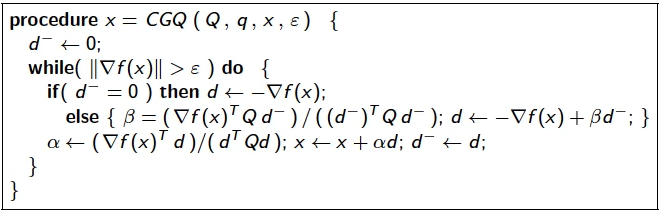
\includegraphics[scale=0.5]{figures/2/chapter2-cgm.png}
    \caption{Conjugate Gradient method.}
    \label{fig:chapter2-cgm}
\end{figure}
\par A powerful property of this algorithm is that it ends in at most $n$ iterations. This is because at each iteration we are minimising over a subset of $k \leq n$ dimensions. Actually, the algorithm can even finish in strictly less than $n$ iterations. This has to do with how are the eigenvalues of $Q$ clustered. If the matrix has $t$ eigenvectors that have equal or almost equal eigenvalues, those $t$ vectors will be killed in just one iteration. In other words, we will minimise along all $t$ directions in just one step. So if we have matrices of 10 thousands variables, but only 10 different eigenvalues, then the algorithm will find the optimum in just 10 iterations. This is very powerful property because what we could do is to do some preconditioning on the initial matrix Q. For instance multiply it with some matrix that cluster the eigenvalues together.
\par The interesting idea is that all this idea can be used also in case of non linear objective function (see figure \ref{fig:chapter2-cgm_nl}). The only difference is that we don't have a closed formula for $\alpha$. No, it is not an error. Look closely at $\beta$ and you will see that the second expression of $\beta$ does not have anything to do with $Q$. Unfortunately we can't say the same for $\alpha$. So we need the saint ways of the line search. This non linear version of Conjugate Gradient with this particular $\beta$ closed formula is called \textbf{Fletcher Reeves method}.
\begin{figure}
    \centering
    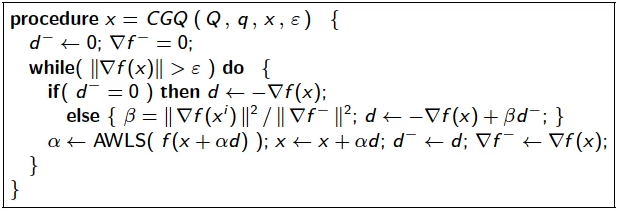
\includegraphics[scale=0.54]{figures/2/chapter2-cgm_nl.png}
    \caption{Conjugate Gradient method for non linear objective function.}
    \label{fig:chapter2-cgm_nl}
\end{figure}
\par There are more ways to compute $\beta$. And of course each one has its own positive and negative sides. In particular there are some formulas that are identical to the one that we have seen in quadratic case, while very different in the non linear case.
\subsection{Convergence and efficiency}
\par The convergence of conjugate gradient method is not trivial and it highly depends on $\beta$. Turns our that for some formulas, it may even not be sufficient to assure Armijo-Wolfe in order to have a descent direction.
\par Sometimes it is also suggested to ``restart'' the direction. Meaning that at a certain point, do not employ the deflected gradient, but just take a plain gradient and deflected gradient from the next iteration.
\par The convergence of conjugate gradient is rather good. It has an \textit{$n$ step quadratic} convergence. Meaning that each $n$ steps the convergence is approximately quadratic. If you think about it, conjugate gradient method minimises optimally a quadratic function in $n$ steps.
%
%
%
\section{Heavy Ball Gradient}
\par It all starts with the following point update:
\begin{equation}
    x^{i+1} = x^i - \alpha \nabla f(x^i) + \beta^i (x^i - x^{i-1})
\end{equation}
\par This method is called Heavy Ball because it is as if $x_i$ was a heavy ball and the gradient is something like a force that wants to steer it away. But since the ball is heavy, it cannot change immediately the direction to 90 degree but it takes time. This is why $\beta$ is called momentum.
\par This is not a descent algorithm. For this reason no one is guaranteeing that each iteration the function is monotonically decreasing. For this reason, the convergence analysis is quite complicated and we won't go into the details.
\par In case of strongly convex function, i.e. $(\lambda^n = u) I \preceq \nabla^2 f(x) \preceq (\lambda^1 = L) I$, actually $\alpha$ and $\beta$ can be estimated:
\begin{align}
    &\alpha = \frac{4}{(\sqrt{\lambda^1} + \sqrt{\lambda^n})^2}\\
    &\beta = \max\{|1-\sqrt{\alpha \lambda^n}|,|1-\sqrt{\alpha \lambda^1}|\}^2
\end{align}
With this choices that we do not prove because it takes a lot of algebra and math, we get the following result:
\begin{equation}
    \Vert x^{i+1} - x^* \Vert \leq (\frac{\sqrt{\lambda^1} - \sqrt{\lambda^1}}{\sqrt{\lambda^1} + \sqrt{\lambda^1}}) \Vert x^{i} - x^* \Vert
\end{equation}
Note that in case of the gradient, the two differences in the norm are in the output space, while here we are getting the difference in the input space. This is a stronger result. This is not a surprising result because strongly convex means just one minimum and the level sets are compact, the best possible situation.
\par The other important difference with the gradient is that we have the square roots. It may seem not a big deal but, square root of the biggest eigenvalue lowers the value of the difference a lot. This means that the expression is nearer to 1, which translates into better convergence. This is the reason why many use Heavy Ball gradient instead of the simple plain gradient.
%
%
%
\section{Accelerated Gradient}
\par There is a version of Heavy Ball gradient that is actually better and it is called \textbf{accelerated gradient} (see figure \ref{fig:chapter2-ag}). It is only for convex functions. This algorithm is obtained from a sophisticated theoretical analysis so will just go through it very quickly.
%
%
%
\section{$< \nabla$ methods}
\par Up until now we have assumed to have the gradient. We can use the gradient method, if we want something faster we can use more than gradient methods. But what if we don't have gradient? What if the function is non differentiable or it is just too difficult to compute the gradient?
%
\subsection{Machine Learning applications}
\par Let us first motivate why we need less than gradient methods. One of the direct application is Machine Learning. In machine learning one has a set of inputs $X = [X^i \subset \mathcal{X}]_{i \in I}$ (it is a matrix) for a given $I = \{1,...,m\}$ and a corresponding set of outputs $Y = [y_i]_{i \in I}$ (a vector). Then one usually wants to devise a mapping function $\Phi : \mathcal{X} \rightarrow \mathcal{F}$ from the space of inputs to the space of features, such that:
\begin{equation}
    \min \{\sum_{i \in I} L(y^i, \Phi(X^i) \cdot w) : w \in \mathbb{R}^n\}
\end{equation}
where $L(\cdot,\cdot)$ is a \textbf{loss function}. In other words, one wants to minimise the loss function, that is a function that computes the distance of the observed outputs from the true outputs.
\par If the loss function is simply the two norm, it becomes the least squares problem:
\begin{equation}
    D
\end{equation}
Note that in ML one has $m$ observations and $n$ weights and usually $m \gg n$. So in case of least squares, we are summing a lot of stuff. So what is that people usually do? Usually the inputs are drawn randomly from some distribution and hopefully they are independently distributed. This means that a small subset of the whole set of observation could be as well as representative. So this is what actually people do. Take a small subset, compute the gradient for that small subset and treat it as it was the gradient of the whole function. So two important questions arise now. How do I choose the subset, and how many do I need? This method takes name of \textbf{stochastic gradient descent} or \textbf{incremental gradient}.
\par Typically, this is not end of story. Convergence may be very hard to achieve. It is for this reason that one usually \textbf{regularise} the objective function:
\begin{equation}
    \min \{\sum_{i \in I} L(y^i, \Phi(X^i) \cdot w) + \mu \Omega(w) : w \in \mathbb{R}^n\}
\end{equation}
$\mu$ is a hyper parameter to decide empirically, $\Omega(w)$ is the regulariser, which is usually $\Omega(w) = \Vert w \Vert_1$ called \textbf{lasso}. Actually, people would like to have 0 norm instead of 1 norm. This is because 0 norm would count how many features are used in the objective function. The problem is that 0 norm is not convex thus it would make the overall problem not convex. So the best convex approximation of the 0 norm is the 1 norm. Unfortunately, 1 norm is not differentiable. This is why of this topic now :).
%
\subsection{Subgradient methods}
\par Remember what a subgradients are:
\begin{equation}
    g \in \partial f(x) \equiv f(y) \geq f(x) + g(y - x), \forall y \in \mathbb{R}^n
\end{equation}
Basically all the functions tangent to the kinks whose epigraph contains entirely the epigraph of the objective function. Each opposite of the subgradient points towards the half space where the optimal solution is located. So going along the direction of one of the opposite of the subgradient should bring us closer to the optimal solution, provided that we do the right step. So the question is: what is the right step?


\section{$> \nabla$ methods}
\par In this section we are going to examine the so called ``more than Gradient methods''. The name comes from the fact that these approaches does not necessarily require to go \textit{strictly} in the opposite direction of the gradient. As we will see, as long as we are going in a descent direction, we are going well.
\par Let us recap briefly what does it mean descent direction and why we selected the opposite of the gradient as the king of such directions. A direction is a descent direction if:
\begin{equation}
    \langle \nabla f(x), d \rangle < 0
\end{equation}
but what does it mean actually? Remember what is the definition of the scalar product:
\begin{equation}
    \langle \nabla f(x), d \rangle = \lVert \nabla f(x) \rVert \lVert d \rVert \cos (\theta)
\end{equation}
where $\theta$ is the angle between $d$ and $\nabla f(x)$. From the moment that both $\lVert d \rVert$ and $\lVert \nabla f(x) \rVert$ are positive (a norm is always $\leq 0$), the only factor that influences the sign of the scalar product is the cosine $\cos(\theta)$. Accordingly, if we set gradient to be the direction of the $x$ asix, as long as the direction $d$ is pointing in the same direction of the $x$ asix, the cosine will be positive. The opposite for the negative value. Thus, the maximum negative value is when the angle $\theta$ is $\pi$, i.e. $\cos(\pi) = -1$, i.i.e. $d = - \nabla f(x)$.
\par Nevertheless, as long as $\cos(\theta) < 0$ we are going down. It is just the matter of a factor $\in [-1,0)$. Provided that the angle is not too far from $\pi$ (or equivalently too small), we can expect that the methods that we are going to present converge. And indeed they do. There is a general result regarding these kind of methods, we announce it without proving it:
\begin{theorem}
    Suppose we have a non unbounded function $f \in C^1$ with $\nabla f$ Lipschitz. Then:
    \[
        (A) \cap (W') \Rightarrow \sum_{i=1}^{\infty} \cos^2(\theta_i) \lVert \nabla f(x_i) \rVert^2 < \infty
    \]
\end{theorem}
This result basically says that, as long as our angle $\theta_i$ is bounded away from 0, we will converge. Note that: if an infinite sequence converges then $\{a_i\} \rightarrow 0$, but not conversely, i.e. a converging sequence to 0 does not imply a converging infinite sum. In our case, actually, it is also possible to converge even if $\cos(\theta)$ is not bounded away from 0, i.e. $cos(\theta) \approx 0$, provided that this does not happen to fast in the series.
%
%
%
\subsection{Newton's Method}
\par Instead of using just the first order model for $f$, we the second order, i.e. quadratic model. Assume for now that the Hessian is positive definite:
\[
    \nabla ^ 2 f(x_i) \succ 0
\]
then exists the minimum of the second order model:
\[
    f(x_i) + \nabla f(x_i) (x-x_i) + \frac{1}{2} (x-x_i)^{T} \nabla ^ 2 f(x_i) (x-x_i)
\]
We can then compute the Newton's direction by:
\begin{align}
    & \nabla f(x) \approx \nabla f(x_i) (x-x_i) + \frac{1}{2} (x-x_i)^{T} \nabla ^ 2 f(x_i) (x-x_i)\\
    & \nabla f(x) = 0\\
    & \nabla f(x_i) (x-x_i) + \frac{1}{2} (x-x_i)^{T} \nabla ^ 2 f(x_i) (x-x_i) = 0\\
    & x = x_i - [\nabla ^ 2 f(x_i)] ^ {-1} \nabla f(x_i)
\end{align}
Thus the direction is given by $- [\nabla ^ 2 f(x_i)] ^ {-1} \nabla f(x_i)$ with $\alpha_i = 1$.
\par Thus the Newton's method is just take a unitary step size along the direction $- [\nabla ^ 2 f(x_i)] ^ {-1} \nabla f(x_i)$.
\par We have seen that Newton converges superlinearly and quadratically in the tail of the convergence:
\begin{align*}
    &f \in C^3 \wedge x_{\star} \text{ saddle point } \wedge \nabla ^ 2 f(x_{\star}) \succ 0 \Rightarrow\\
    &\exists \mathcal{B}(x_{\star}, r) : (x_1 \in \mathcal{B}(x_{\star}, r) \Rightarrow \{x_i\} \rightarrow x_{\star} \text{ quadratically})
\end{align*}
This means that if the algorithm starts in a ball around the saddle point, it will converge quadratically to the optimum point. The issue is that we cannot know whether or not we are starting in the proximity of the optimal point. Not a big deal: we could try to run Netwon's method and in case we do not get the quadratic convergence we restart by using the standard Armijo-Wolfe line search.
\par The function must have a positive definite Hessian since we need to invert it to get the direction. The direction obtained is surely a descent direction as we can verify it by the following:
\[
    d_i \nabla f(x_i) = - \nabla f(x_i)^{T} [\nabla^2 f(x_i)]^{-1} \nabla f(x_i) < 0
\]
where the last inequality follows from the fact that the Hessian is a symmetric positive definite matrix.
\par We can interpret Newton's method from another point of view (\textbf{Space Dilatation}). Suppose Hessian $Q$ is symmetric and positive definite. Then we can find a matrix $R$ such that $Q = R^TR$ and $R = \sqrt{Q}$. We are sure that such an $R$ exists and that it is symmetric. Thus:
\[
    Q = H \Lambda H^T \Rightarrow R = H \sqrt{\Lambda} H^T
\]
infact:
\[
    R^TR = (H \sqrt{\Lambda} H^T)^T H \sqrt{\Lambda} H^T = H \sqrt{\Lambda} H^T H \sqrt{\Lambda} H^T = H \Lambda H^T
\]
Suppose now:
\[
    f(x) = \frac{1}{2} x^T Q x + q^T x
\]
the gradient of this function is:
\[
    \nabla f(x) = Qx + q
\]
and the direction is:
\[
    d = -Q^{-1}q
\]
Since we have $Q = R^TR$, we can rewrite the function as:
\[
    f(x) = \frac{1}{2} x^T R^TR x + q^Tx
\]
We then set $y = Rx$ and proceed like:
\[
    f(y) = \frac{1}{2} y^T I y + q^T R^{-1}y
\]
with the gradient:
\[
    \nabla f(y) = y + R^{-1}q
\]
and the direction:
\[
    d = -R^{-1}q
\]
As we can see, the Hessian of this new function is surely symmetric positive definite (identity matrix). Moreover, $\lambda_n(I) = \lambda_1(I)$ which means that the Newton's method \textit{finishes in one iteration}. 
\par Let us now speak about Newton's convergence. We suppose our function is convex with gradient Lipschitz continuous. This implies the following:
\[
    uI \leq \nabla ^ 2 f \leq LI
\]
We can now prove that it is convergent provided that $\cos(\theta)$ does not go to 0 too fast, otherwise we will not go in the descent direction.
\begin{proof}
We want to prove the following:
\[
    \cos(\theta_i) \leq 0
\]
Since the dot product between $\nabla f(x_i)$ and $d_i$ must be negative. Thus we need to show that:
\[
    \frac{\langle \nabla f(x_i), d_i \rangle}{\lVert \nabla f(x_i) \rVert \lVert d_i \rVert} \leq 0
\]
Let us start with the numerator:
\[
    d_i = - [\nabla ^ 2 f(x_i)]^{-1} \nabla f(x_i) \Rightarrow [\nabla ^ 2 f(x_i)] d_i = - \nabla f(x_i)
\]
we now multiply both sides by $- d_i^T$:
\[
    - d_i^T[\nabla ^ 2 f(x_i)] d_i = d_i^T \nabla f(x_i)
\]
Since the Hessian is symmetric we can use the Spectra decomposition:
\[
    \lambda_n \lVert d_i \rVert ^ 2 \leq d_i^T[\nabla ^ 2 f(x_i)] d_i \leq \lambda_1 \lVert d_i \rVert ^ 2
\]
But be careful, we have a minus up there, thus:
\[
    - \lambda_n \lVert d_i \rVert ^ 2 \geq - d_i^T[\nabla ^ 2 f(x_i)] d_i \geq - \lambda_1 \lVert d_i \rVert ^ 2
\]
So we then obtain:
\[
    d_i^T \nabla f(x_i) = - d_i^T[\nabla ^ 2 f(x_i)] d_i \leq - \lambda_n \lVert d_i \rVert ^ 2
\]
As for the denominator, we get:
\[
    \lVert \nabla f(x_i) \rVert = \lVert \nabla ^ 2 f(x_i) d_i \rVert
\]
from the definition of the Newton's direction. Now we use the Cauchy-Schwartz inequality:
\[
    \lVert \nabla f(x_i) \rVert = \lVert \nabla ^ 2 f(x_i) d_i \rVert \leq \lVert \nabla ^ 2 f(x_i) \rVert \lVert d_i \rVert = \lambda_1 \lVert d_i \rVert
\]
where the last equality follows from the fact that the norm of the Hessian, by spectral decomposition, is the norm of the diagonal matrix $\Lambda$, i.e. $\lambda_1$.
\par We can now give an upper bound for $\cos(\theta_i)$:
\[
    \cos(\theta_i) = \frac{\langle \nabla f(x_i), d_i \rangle}{\lVert \nabla f(x_i) \rVert \lVert d_i \rVert} = \frac{\nabla d_i^T f(x_i)}{\lVert \nabla f(x_i) \rVert \lVert d_i \rVert} \leq \frac{- \lambda_n \lVert d_i \rVert ^ 2}{\lambda_1 \lVert d_i \rVert \lVert d_i \rVert} = - \frac{\lambda_n}{\lambda_1} \leq - \frac{u}{L}
\]
Since $u$ and $L$ are strictly positive, we have that the value of cosine is strictly negative.
\end{proof}
\par Newton works very well on convex and strictly convex function. But does it also work with non convex ones? Yes.
\par When we spoke about the convergence above, we did not use the fact that the function is convex really. What we used is the fact that Hessian is positive definite. Thus if our function does not have a positive definite matrix we can perturb it slightly in order to get a close positive definite one. This method is called \textbf{Hessian modification}. We choose the smallest $\epsilon_i$ such that:
\[
    H^i = \nabla ^ 2 f(x_i) + \epsilon_i I \succ 0
\]
Nevertheless, we have a minor numerical issue here. Every $\epsilon_i > - \lambda_n$ will work fine (remember: since $\nabla ^2 f \succ 0$ we know that the smallest eigenvalue is strictly positive). But if $\lambda_n$ is of machine precision order, we could risk to set $\epsilon_i = 0$. We suppose here that this does not occur.
\par Accordingly, we take $\epsilon_i = \max \{0, \delta - \lambda_n\}$ and we solve the following constraint optimisation problem:
\[
    \min_{H_i}\{\lVert H_i - \nabla ^ 2 f(x_i) \rVert_{F} :  H \geq \delta I\}
\]
How can we solve such a problem. Using spectral decomposition of the Hessian:
\[
    \nabla ^ 2 f(x_i) = H \Lambda H^T
\]
We then take:
\[
    H_i = H \bar{\Lambda} H^T
\]
where $\bar{\Lambda}$ has on diagonal $\bar{\gamma}_i = \max \{\lambda_i, \delta\}$.
\par The problem with this approach is that at each iteration we need to invert and factorise. This costs $\mathcal{O}(n^3)$, cubic complexity. That's the reason why we move now to the Quasi-Newton methods.
%
%
%
\subsection{Quasi-Newton Methods}
Quasi-Newton methods can be used if the Hessian is unavailable or is too expensive to compute at every iteration. We do not need actually the exact Hessian in the quadratic model of the function, we just need a positive definite matrix. The model $m$ of our function $f$ then becomes:
\[
    m_i(x) \approx f(x_i) + \nabla f(x_i) (x-x_i) + \frac{1}{2} (x-x_i)^T H_i (x-x_i)
\]
After computing $\nabla f(x_{i+1})$ where $x_{i+1} = x_i + \alpha_i d_i$, we update our model $m$ of $f$ by:
\[
    m_{i+1}(x) \approx f(x_{i+1}) + \nabla f(x_{i+1}) (x-x_{i+1}) + \frac{1}{2} (x-x_{i+1})^T H_i (x-x_{i+1})
\]
The problem is: how can we compute $H^{i+1}$ efficiently. Let us reason about what we want that $H^{i+1}$ satisfy:
\begin{enumerate}
    \item $H^{i+1} \succ 0$
    \item $\nabla m^{i+1}(x_i) = \nabla f(x_i)$, i.e. the gradient in the previous point $x_i$ of the new model must be the same of the previous model in the same point. This is called \textbf{Secant equation}
    \item $\lVert H^{i+1} - H^i \rVert$ is small
\end{enumerate}
Note how the second point can be also written as:
\begin{align*}
    \nabla m^{i+1}(x_{i+1} - x_i) &= f(x_{i+1}) + \nabla f(x_{i+1}) (x_{i+1} - x_i - x_{i+1}) +\\
    &+\frac{1}{2} (x_{i+1} - x_i -x_{i+1})^T H_i (x_{i+1} - x_i -x_{i+1}) =\\
    & = f(x_{i+1}) - \nabla f(x_{i+1}) (x_i) + \frac{1}{2} (- x_i)^T H_i (- x_i) TO FINISH
\end{align*}
\par Let us now see how can we compute such a matrix $H^{i+1}$. We define the following:
\[
    s_i = x_{i+1} - x_i
\]
and
\[
    y_i = f(x_{i+1}) - f(x_i)
\]
Thus we can write:
\[
    H^{i+1}s_i = y_i
\]
We then multiply both sides by $s_i^T$:
\subsection{Conjugate Gradient Method}
\subsection{Deflected Gradient Methods}